\chapter{Evaluation and Analysis}

In the previous chapter, a few approaches that could improve the genetic solver were presented.
The best results give a combination of the genetic solver with added probabilities and parameter tuning.
Other methods like a changeable crossover rate or population without duplicated individuals have less effect on the results.

However, we get valid results only for one problem. What if the problem will be smaller or bigger?
The evaluation was done to find out how all approaches work with different problem sizes. 

\section{Evaluation}
\label{sec:evaluation}

To evaluate the genetic solver, we performed a benchmark. The benchmark set consists of 36 problems. Each problem has different parameters that describe it.
All parameters are:
\begin{itemize}
	\item Software variants - [2, 4] ,
	\item Number of requests - [1, 2, 4],
	\item Component tree depth - [2, 3, 4],
	\item  Resources ratio - [50, 100],
	\item timeout to solve the problem: 5 minutes.
\end{itemize}

This set was tested with several versions of the genetic solver:

\begin{itemize}
	\item basic (B),
	\item basic with tuned parameters (B-T),
	\item without hard-coded parameters and tuning (WHC-T) 
	\item with added parameters (NP),
	\item with added parameters and tuning (NP-T),
	\item with internally changeable crossover rate (ICCR),
	\item with internally changeable crossover rate and tuning (ICCR-T),
	\item without duplicates in the population (WD),
	\item without duplicates in the population and tuning (WD-T).
\end{itemize}

Each version of the genetic solver tries five times to solve each problem.

The benchmark set was run on an Intel Core i7-8700 CPU machine with 64Gb of memory using Fedora Server 29 and OpenJDK 1.8.0 201-b09.

Benchmark trying so solve each task, if a solution was valid, genetic solver start to solve the next problem. If, after five attempts, the genetic solver did not find a valid solution, it proceeded to the next problem.

\begin{figure}
	\centering
	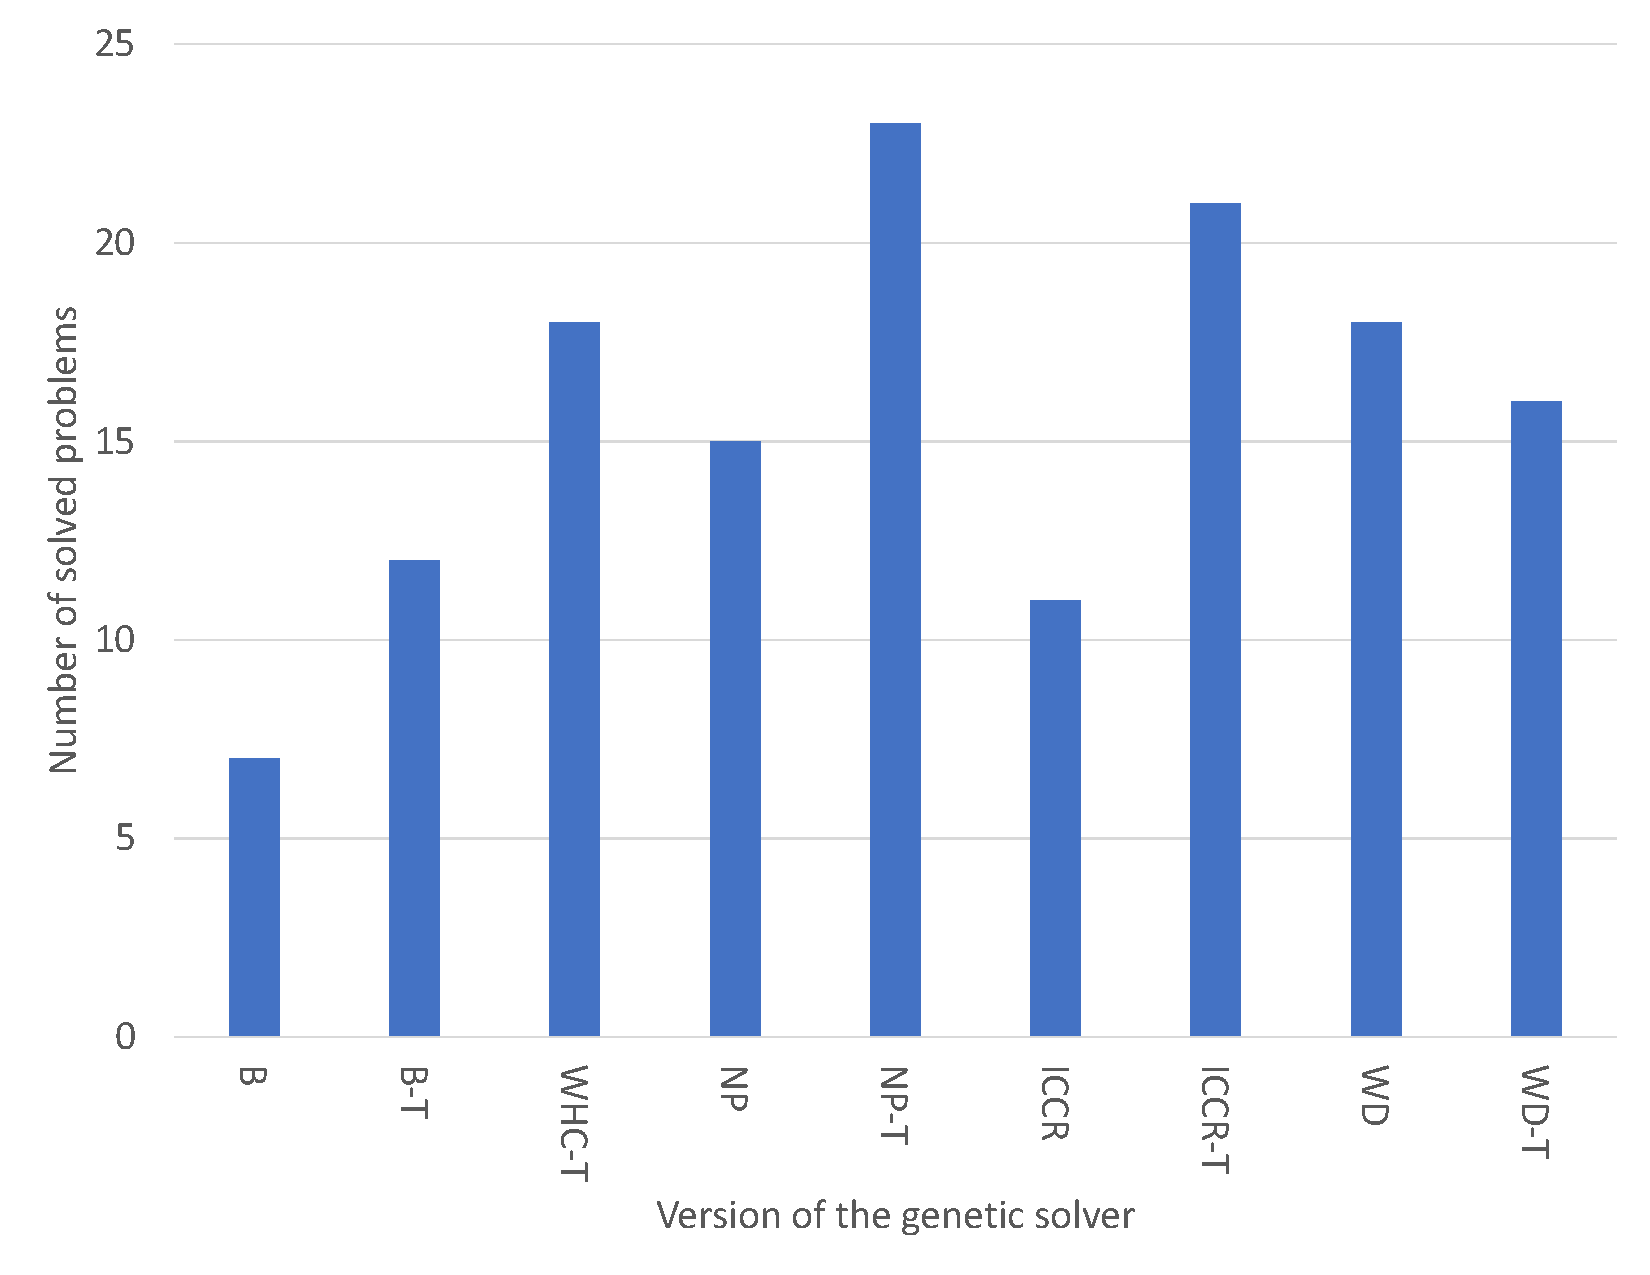
\includegraphics[width=\textwidth]{images/EvaluationNumberOfSolvedProblems.pdf}
	\caption[Number of problems for each version of the genetic solver]{Number of solved problems for each version of the genetic solver}
	\label{fig:EvaluationNumberOfSolvedProblems}
\end{figure}

Figure~\ref{fig:EvaluationNumberOfSolvedProblems} results of the benchmark. For each version of the genetic solver, a vertical bar was built. The height of the bar shows the number of solved problems from the benchmark set. The B version solved the least of problems than any other version. Almost in all cases, parameter tuning increases the number of solved problems. It also confirms the answer to \textbf{RQ1}. 

The comparison of B-T, WHC-T, and NP versions shows that the NP bar is higher than B-T but lower than WHC-T. This comparison confirms the first conclusion from Section~\ref{sec:NP}, that well-designed parameters are important for any algorithm. The combination of parameter engineering and parameter tuning in NP-T gives the best results. The same situation was for one problem in the previous chapter~(Figure~\ref{fig:boxplotsolverNoDuplicates}). 

The WD-T gives worse results than the untuned version. The possible reason for such results is a high value of the \texttt{meu}~(R6) parameter. The result of the benchmark for the ICCR-T version contradicts the results obtained in the last section because the parameter tuning of the ICCR version gives the biggest improvement. In general, benchmark results for a set of 36 MQuAT problems correspond to the results for one problem.

The benchmark also shows that no one version of the genetic solver solved all problems from the set. Table~\ref{tab:ProblemsColorCoding} shows the results of the benchmark in the context of a solved or unsolved problem. Each row describes the result for a specified problem. The problem numbers contain in column \textit{Problem Id}. Black filled cell means that solver solved the problem. Table~\ref{tab:ProblemsColorCoding} also shows ids of problems that unsolved by all versions of the genetic solver.

\begin{table}
	\caption{Problem color coding}\label{tab:ProblemsColorCoding}
	\resizebox{0.8\textwidth}{!}{
	\begin{minipage}[t]{0.5\linewidth}
		\begin{tabular}[t]{c | c | c | c | c | c | c | c | c | c |}
			\rotatebox{90}{Problem Id} & \rotatebox{90}{B} & \rotatebox{90}{B-T} & \rotatebox{90}{WHC-T} & \rotatebox{90}{NP} & \rotatebox{90}{NP-T} & \rotatebox{90}{ICCR} & \rotatebox{90}{ICCR-T} & \rotatebox{90}{WD} & \rotatebox{90}{WD-T} \\
			\hline            
			1 & $\blacksquare$ & $\blacksquare$ & $\blacksquare$ & $\blacksquare$ & $\blacksquare$ & $\blacksquare$ & $\blacksquare$ & $\blacksquare$ & $\blacksquare$ \\ 
			2 & $\square$ & $\square$ & $\blacksquare$ & $\square$ & $\blacksquare$ & $\square$ & $\square$ & $\blacksquare$ & $\blacksquare$  \\
			3 & $\square$ & $\square$ & $\square$ & $\square$ & $\blacksquare$ & $\square$ & $\square$ & $\blacksquare$ & $\square$  \\
			4 & $\square$ & $\blacksquare$ & $\blacksquare$ & $\blacksquare$ & $\blacksquare$ & $\blacksquare$ & $\blacksquare$ & $\blacksquare$ & $\blacksquare$ \\
			5 & $\square$ & $\square$ & $\square$ & $\square$ & $\blacksquare$ & $\square$ & $\blacksquare$ & $\square$ & $\square$ \\
			6 & $\square$ & $\square$ & $\square$ & $\square$ & $\square$ & $\square$ & $\square$ & $\square$ & $\square$ \\
			7 & $\square$ & $\blacksquare$ & $\blacksquare$ & $\blacksquare$ & $\blacksquare$ & $\square$ & $\blacksquare$ & $\blacksquare$ & $\blacksquare$\\
			8 & $\square$ & $\square$ & $\square$ & $\square$ & $\square$ & $\square$ & $\square$ & $\square$ & $\square$ \\
			9 & $\square$ & $\square$ & $\square$ & $\square$ & $\square$ & $\square$ & $\square$ & $\square$ & $\square$ \\
			10 & $\blacksquare$ & $\blacksquare$ & $\blacksquare$ & $\blacksquare$ & $\blacksquare$ & $\blacksquare$ & $\blacksquare$ & $\blacksquare$ & $\blacksquare$ \\
			11 & $\square$ & $\square$ & $\blacksquare$ & $\blacksquare$ & $\blacksquare$ & $\blacksquare$ & $\blacksquare$ & $\blacksquare$ & $\blacksquare$ \\
			12 & $\square$ & $\square$ & $\square$ & $\square$ & $\blacksquare$ & $\square$ & $\blacksquare$ & $\blacksquare$ & $\square$  \\
			13 & $\blacksquare$ & $\blacksquare$ & $\blacksquare$ & $\blacksquare$ & $\blacksquare$ & $\blacksquare$ & $\blacksquare$ & $\blacksquare$ & $\blacksquare$ \\
			14 & $\square$ & $\square$ & $\square$ & $\square$ & $\blacksquare$ & $\square$ & $\blacksquare$ & $\square$ & $\square$  \\
			15 & $\square$ & $\square$ & $\square$ & $\square$ & $\square$ & $\square$ & $\square$ & $\square$ & $\square$ \\
			16 & $\square$ & $\blacksquare$ & $\blacksquare$ & $\blacksquare$ & $\blacksquare$ & $\square$ & $\blacksquare$ & $\square$ & $\blacksquare$ \\
			17 & $\square$ & $\square$ & $\square$ & $\square$ & $\square$ & $\square$ & $\square$ & $\square$ & $\square$ \\
			18 & $\square$ & $\square$ & $\square$ & $\square$ & $\square$ & $\square$ & $\square$ & $\square$ & $\square$ \\
			\hline
		\end{tabular} %
	\end{minipage}
	%\setlength{\tabcolsep}{0.05cm}
	%\renewcommand{\arraystretch}{0}
	\begin{minipage}[t]{0.49\linewidth}
		\begin{tabular}[t]{c | c | c | c | c | c | c | c | c | c}
			\rotatebox{90}{Problem Id} & \rotatebox{90}{B} & \rotatebox{90}{B-T} & \rotatebox{90}{WHC-T} & \rotatebox{90}{NP} & \rotatebox{90}{NP-T} & \rotatebox{90}{ICCR} & \rotatebox{90}{ICCR-T} & \rotatebox{90}{WD} & \rotatebox{90}{WD-T} \\
			\hline            
			19 & $\blacksquare$ & $\blacksquare$ & $\blacksquare$ & $\blacksquare$ & $\blacksquare$ & $\blacksquare$ & $\blacksquare$ & $\blacksquare$ & $\blacksquare$\\
			20 & $\square$ & $\square$ & $\blacksquare$ & $\blacksquare$ & $\blacksquare$ & $\blacksquare$ & $\blacksquare$ & $\blacksquare$ & $\blacksquare$ \\
			21 & $\square$ & $\square$ & $\square$ & $\square$ & $\blacksquare$ & $\square$ & $\blacksquare$ & $\square$ & $\square$ \\
			22 & $\blacksquare$ & $\blacksquare$ & $\blacksquare$ & $\square$ & $\blacksquare$ & $\blacksquare$ & $\blacksquare$ & $\blacksquare$ & $\blacksquare$ \\
			23 & $\square$ & $\square$ & $\blacksquare$ & $\blacksquare$ & $\blacksquare$ & $\square$ & $\blacksquare$ & $\blacksquare$ & $\square$ \\
			24 & $\square$ & $\square$ & $\square$ & $\square$ & $\square$ & $\square$ & $\square$ & $\square$ & $\square$ \\
			25 & $\square$ & $\square$ & $\blacksquare$ & $\blacksquare$ & $\blacksquare$ & $\square$ & $\blacksquare$ & $\square$ & $\blacksquare$ \\
			26 & $\square$ & $\square$ & $\square$ & $\square$ & $\square$ & $\square$ & $\square$ & $\square$ & $\square$ \\
			27 & $\square$ & $\square$ & $\square$ & $\square$ & $\square$ & $\square$ & $\square$ & $\square$ & $\square$ \\
			28 & $\blacksquare$ & $\blacksquare$ & $\blacksquare$ & $\blacksquare$ & $\blacksquare$ & $\blacksquare$ & $\blacksquare$ & $\blacksquare$ & $\blacksquare$ \\
			29 & $\square$ & $\blacksquare$ & $\blacksquare$ & $\blacksquare$ & $\blacksquare$ & $\blacksquare$ & $\blacksquare$ & $\blacksquare$ & $\blacksquare$ \\
			30 & $\square$ & $\square$ & $\square$ & $\square$ & $\square$ & $\square$ & $\square$ & $\square$ & $\square$ \\
			31 & $\blacksquare$ & $\blacksquare$ & $\blacksquare$ & $\blacksquare$ & $\blacksquare$ & $\blacksquare$ & $\blacksquare$ & $\blacksquare$ & $\blacksquare$ \\
			32 & $\square$ & $\square$ & $\blacksquare$ & $\blacksquare$ & $\blacksquare$ & $\square$ & $\blacksquare$ & $\blacksquare$ & $\square$ \\ 
			33 & $\square$ & $\square$ & $\square$ & $\square$ & $\square$ & $\square$ & $\square$ & $\square$ & $\square$ \\
			34 & $\square$ & $\blacksquare$ & $\blacksquare$ & $\square$ & $\blacksquare$ & $\square$ & $\blacksquare$ & $\blacksquare$ & $\blacksquare$ \\
			35 & $\square$ & $\square$ & $\square$ & $\square$ & $\square$ & $\square$ & $\square$ & $\square$ & $\square$ \\
			36 & $\square$ & $\square$ & $\square$ & $\square$ & $\square$ & $\square$ & $\square$ & $\square$ & $\square$ \\
			\hline
		\end{tabular} %
	\end{minipage}
	}
	\mbox{$\blacksquare$: solved, $\square$: unsolved}
\end{table}

Unsolved tasks are presented in Table~\ref{tab:UnsolvedProblems}. It shows parameters that specified the problem. We can see, there are a few types of unsolved problems are exist. All versions of the genetic solver could not solve the problem that contains two or more requests, and the depth is three or more. The exception for this definition is a problem number 30. It has one request and depth four, but it also has variants four and resources - 100 and genetic solvers could not solve it.

\begin{itemize}
	\item Software variants - [2, 4] ,
	\item Number of requests - [1, 2, 4],
	\item Component tree depth - [2, 3, 4],
	\item Resources ratio - [50, 100],
	\item timeout to solve the problem: 5 minutes.
\end{itemize}

\begin{table}
	\centering
	\caption{Not solved problems}\label{tab:UnsolvedProblems}
	%\resizebox{0.6\textwidth}{!}{
		\begin{tabular}{c c c c c}
			\hline
			Problem Id & Software variants & umber of requests & Component tree depth & Resources ratio \\
			\hline            
			6 & 2 & 2 & 4 & 50 \\
			8 & 2 & 4 & 3 & 50 \\
			9 & 2 & 4 & 4 & 50 \\
			15 & 2 & 2 & 4 & 100 \\
			17 & 2 & 4 & 3 & 100 \\
			18 & 2 & 4 & 4 & 100 \\
			24 & 4 & 2 & 4 & 50 \\
			26 & 4 & 4 & 3 & 50 \\
			27 & 4 & 4 & 4 & 50 \\
			30 & 4 & 1 & 4 & 100 \\
			33 & 4 & 2 & 4 & 100 \\
			35 & 4 & 4 & 3 & 100 \\
			36 & 4 & 4 & 4 & 100 \\
			\hline
		\end{tabular}
	%}
\end{table}

If a genetic solver could solve some problems, then solutions have a quality.
Let us now discuss the quality of the received results. Figure~\ref{fig:EnergyPercentage} shows the percentage of the deviation from the optimum for problems that solved by all versions of the genetic solver. The optimum values for problems received by the ILP solver. If the percentage of the deviation is zero, that means that the received solution is \textbf{optimal}. The max deviation is near 30\% for the B version with problem 31. However, other versions give solutions with deviation from optimal that less than 10\% or even optimal solutions for the NP-T version. There are high deviations from optimum in problems number 13 for tuned versions of the genetic solver such as B-T, NP-T, ICCR-T, and WD-T. Nevertheless, WHC-T and untuned versions give a near-optimal solution with minimal deviation. The ICCR version gives a much higher percentage of deviation than other versions in problem 19.

\begin{figure}
	\centering
	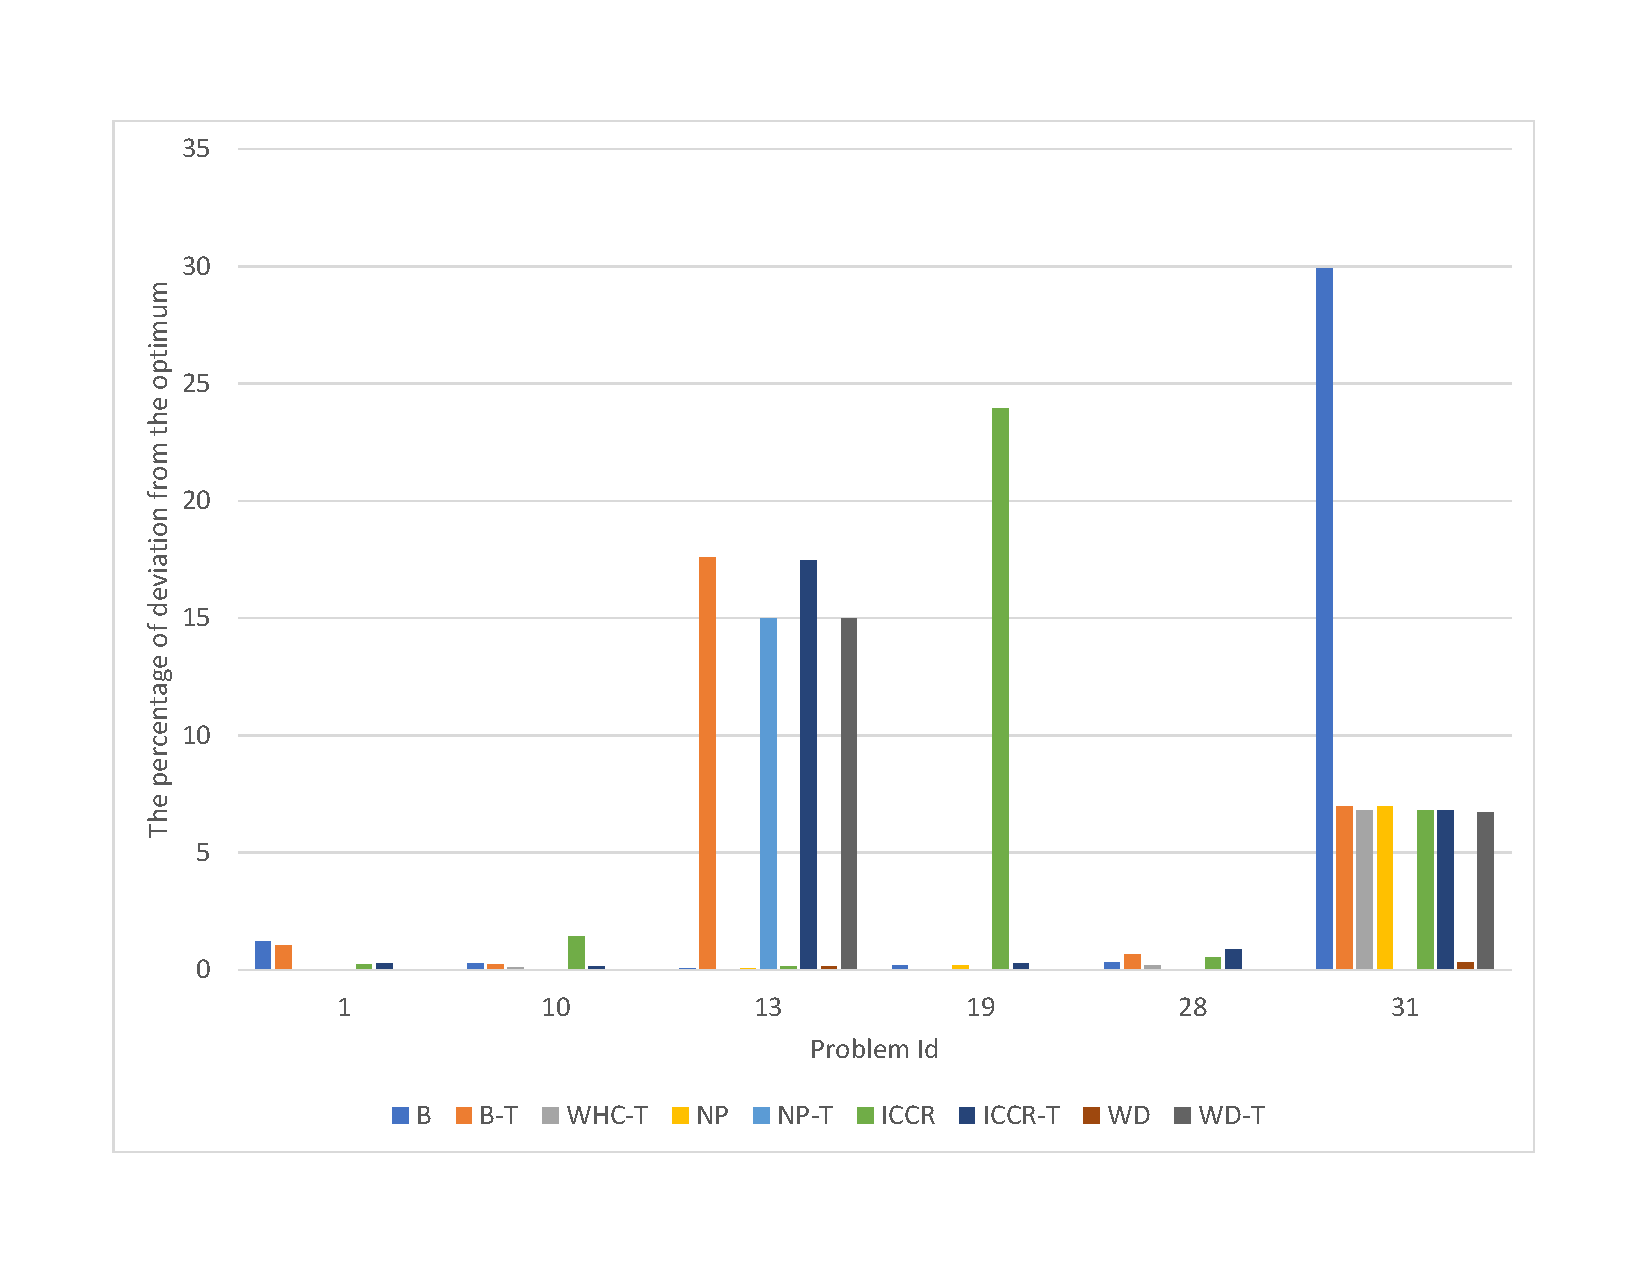
\includegraphics[width=\textwidth]{images/EnergyPercentage.pdf}
	\caption[]{}
	\label{fig:EnergyPercentage}
\end{figure}

Figure~\ref{fig:EnergyPercentage} also shows that the deviation is increasing for big size problems. To confirm that fact, we take two problems with different sizes~(Figures~\ref{fig:SmallMediumProblemEnergy}). These problems solved by all versions of the genetic solver except the B version. Figure~\ref{fig:SmallProblemEnergy} shows the percentage of deviation from optimum for a small size problem. This problem's parameters are:
\begin{itemize}
	\item Software variants: 2,
	\item Number of requests: 2,
	\item Component tree depth: 2,
	\item Resources ratio: 50,
	\item timeout to solve the problem: 5 minutes.
\end{itemize}

The quality of results for the problem is near-optimal because the deviation is less than one percent. The NP-T and WD-T versions give an optimal solution for the problem.

Figure~\ref{fig:MediumProblemEnergy} shows the percentage of deviation from optimum for a bigger size problem. This problem's parameters are:
\begin{itemize}
	\item Software variants: 4,
	\item Number of requests: 1,
	\item Component tree depth: 3,
	\item Resources ratio: 100,
	\item timeout to solve the problem: 5 minutes.
\end{itemize}


The quality of results in a case of the bigger problem is much worse. The minimal deviation is 35\% for the NP-T version because the deviation is less than one percent. The NP-T and WD-T versions give an optimal solution for the problem. The WD and WD-T versions give less number of valid solutions, but with better quality. The quality of the solution from other solvers is lower because the percentage of the deviation is more than 100\%. The reason why the quality of solutions is decreasing with a bigger size of the problem could be a higher number of hardware resources. The higher number of resources means that more hardware resources could satisfy the requirements of the software component. The genetic solver could not find best-suited resources for requested components, and as a result, quality is decreasing. 


\begin{figure}
	\centering
	\begin{subfigure}{0.45\textwidth}
		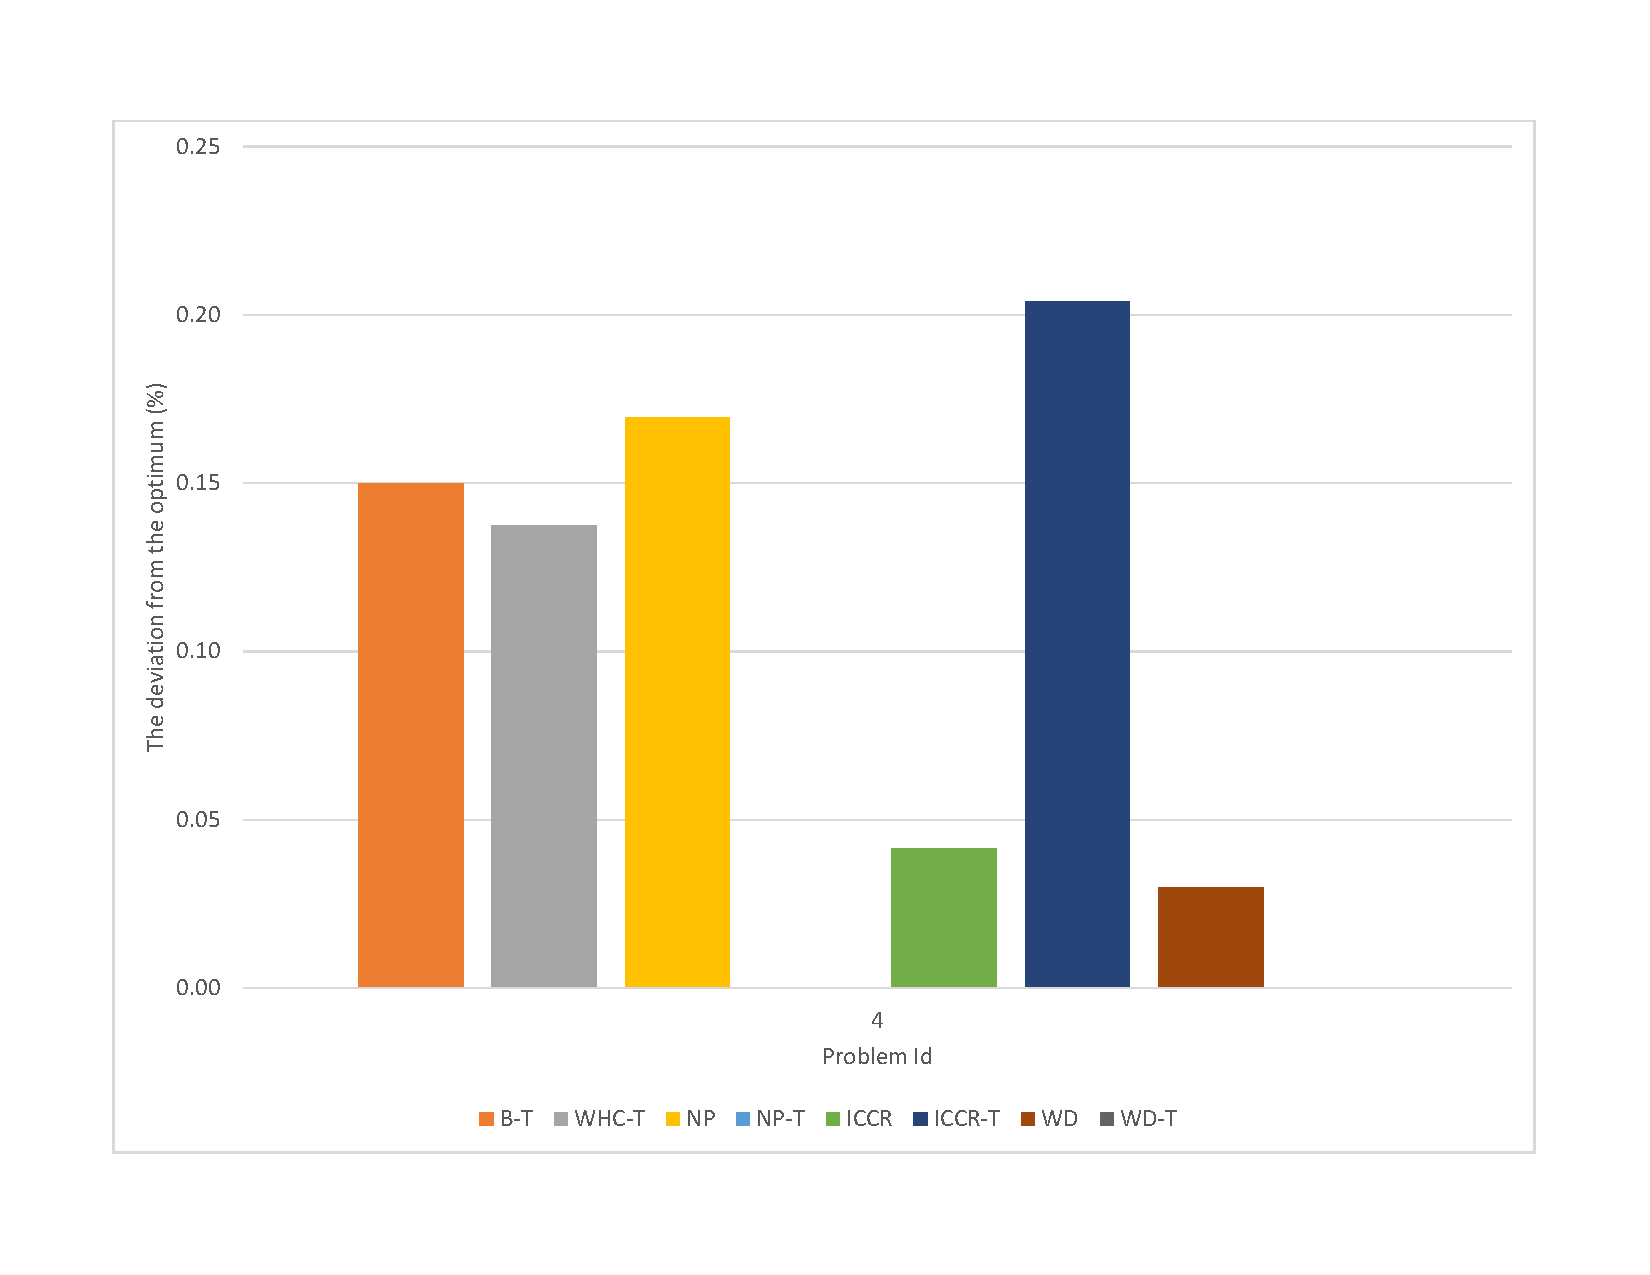
\includegraphics[width=\textwidth]{images/EnergyDeviationSmallProblem.pdf}
		\caption{$y=x$}
		\label{fig:SmallProblemEnergy}
	\end{subfigure}
	\hfill
	\begin{subfigure}{0.45\textwidth}
		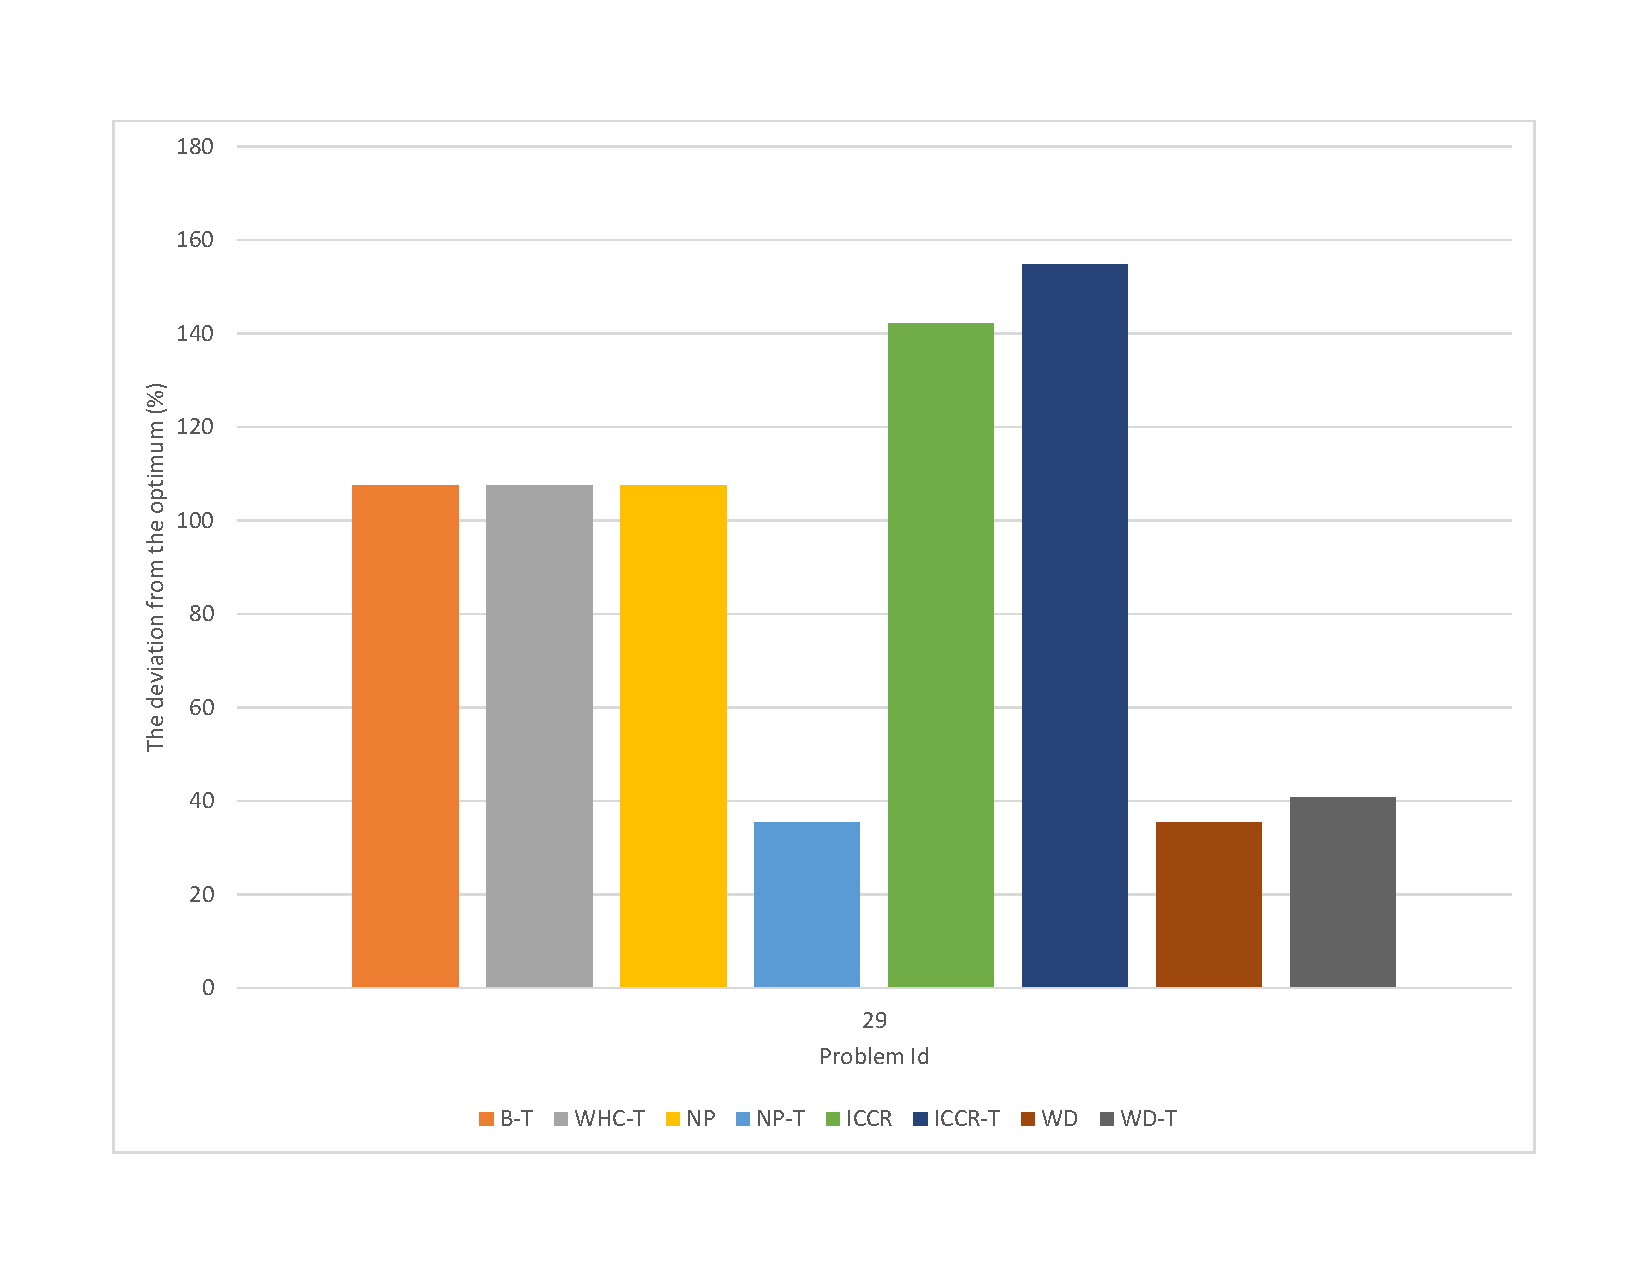
\includegraphics[width=\textwidth]{images/EnergyDeviationMediumProblem.pdf}
		\caption{$y=x$}
		\label{fig:MediumProblemEnergy}
	\end{subfigure}    
	\caption{Three simple graphs}
	\label{fig:SmallMediumProblemEnergy}    
\end{figure}


This section shows that modification that we made improve the results of the genetic solver. The NP-T version solved three times more problems than the B version. We evaluated the quality of solutions. As a result of the quality evaluation, we make two conclusions. First, modified versions of the genetic solver also improve the quality of the results. Second, the quality is decreasing for a bigger size of the problem.
However, there are problems from the set that could not be solved by the genetic solver.


\section{Analysis}

Benchmark showed that a genetic solver could not solve all MQuAT problems from the evaluation set.
In this section, we presented an analysis of results, reasons why described in Chapter~\ref{chapter:Implementation} approaches, and optimizations have lower efficiency that we need.

Firstly, let us discuss the reasons why modifications that we made improve the genetic solver. After that, we will concentrate on the reasons why not all tasks could be solved.

There are a few reasons why the genetic solver with our modifications could solve more problems than the B version. First of all, parameter tuning was performed for all versions. Optimized values of parameters give better results, as it showed in the previous section. The second reason are new probabilities that we added in Section~\ref{sec:NP}. These probabilities give a possibility to change the position of the crossover and mutation points randomly, and as a result, the genetic solver gives results that a bit worse than parameter tuning. 

Nevertheless, not all tasks were solved. One of the reasons for such a result is parameter tuning. We optimized parameters for a specific problem that we described at the beginning of Chapter~\ref{chapter:Implementation}.

Obtained results could be described with a \textbf{"no free lunch" (NFL) theorem}\cite{wolpert1996, wolpert1997}. It says that if an algorithm works well with a certain class of tasks, then it must pay for it with a deterioration in performance on the set of all remaining problems.

Another reason that we optimize parameters without knowledge about dependencies between them. Parameters that we found or added did not fit well for our goals. Let us analyze earlier discussed parameters.

We start an analysis with search space representation. For this representation, we performed measurements for more than three thousand configurations using BRISE in the Search space exploration mode with the NP version of the genetic solver. This mode was described in Section~\ref{sec:BRISE}. For this type of analysis, we use the same problem as in Chapter~\ref{chapter:Implementation} and it has parameter values:
\begin{itemize}
	\item Software variants: 10,
	\item Number of requests: 15,
	\item Component tree depth: 2,
	\item Resources ratio: 5,
	\item timeout to solve the problem: 5 minutes.
\end{itemize}

The search space representation for the SPEA2 selector as a parallel coordinates plot showed in Figure~\ref{fig:SearchSpaceViewFull}.
Each parameter is represented in the plot as a vertical line that contains all possible values of the parameter. Each configuration that was measured showed on the plot as a line that connects all values that describe itself. The last vertical line and the color shows the number of contract violations that give the configuration. The more dark color means fewer contract violations and vise versa, the lighter color gives a higher number of contract violations.

\begin{figure}
	\centering
	\includegraphics[width=\textwidth]{images/SPEA2.pdf}
	\caption[]]{}
	\label{fig:SearchSpaceViewFull}
\end{figure}

Figure~\ref{fig:SearchSpaceViewFull} shows all values of parameters could give "good" and "bad" results. There are no visible dependencies between parameters. 

\begin{figure}
	\centering
	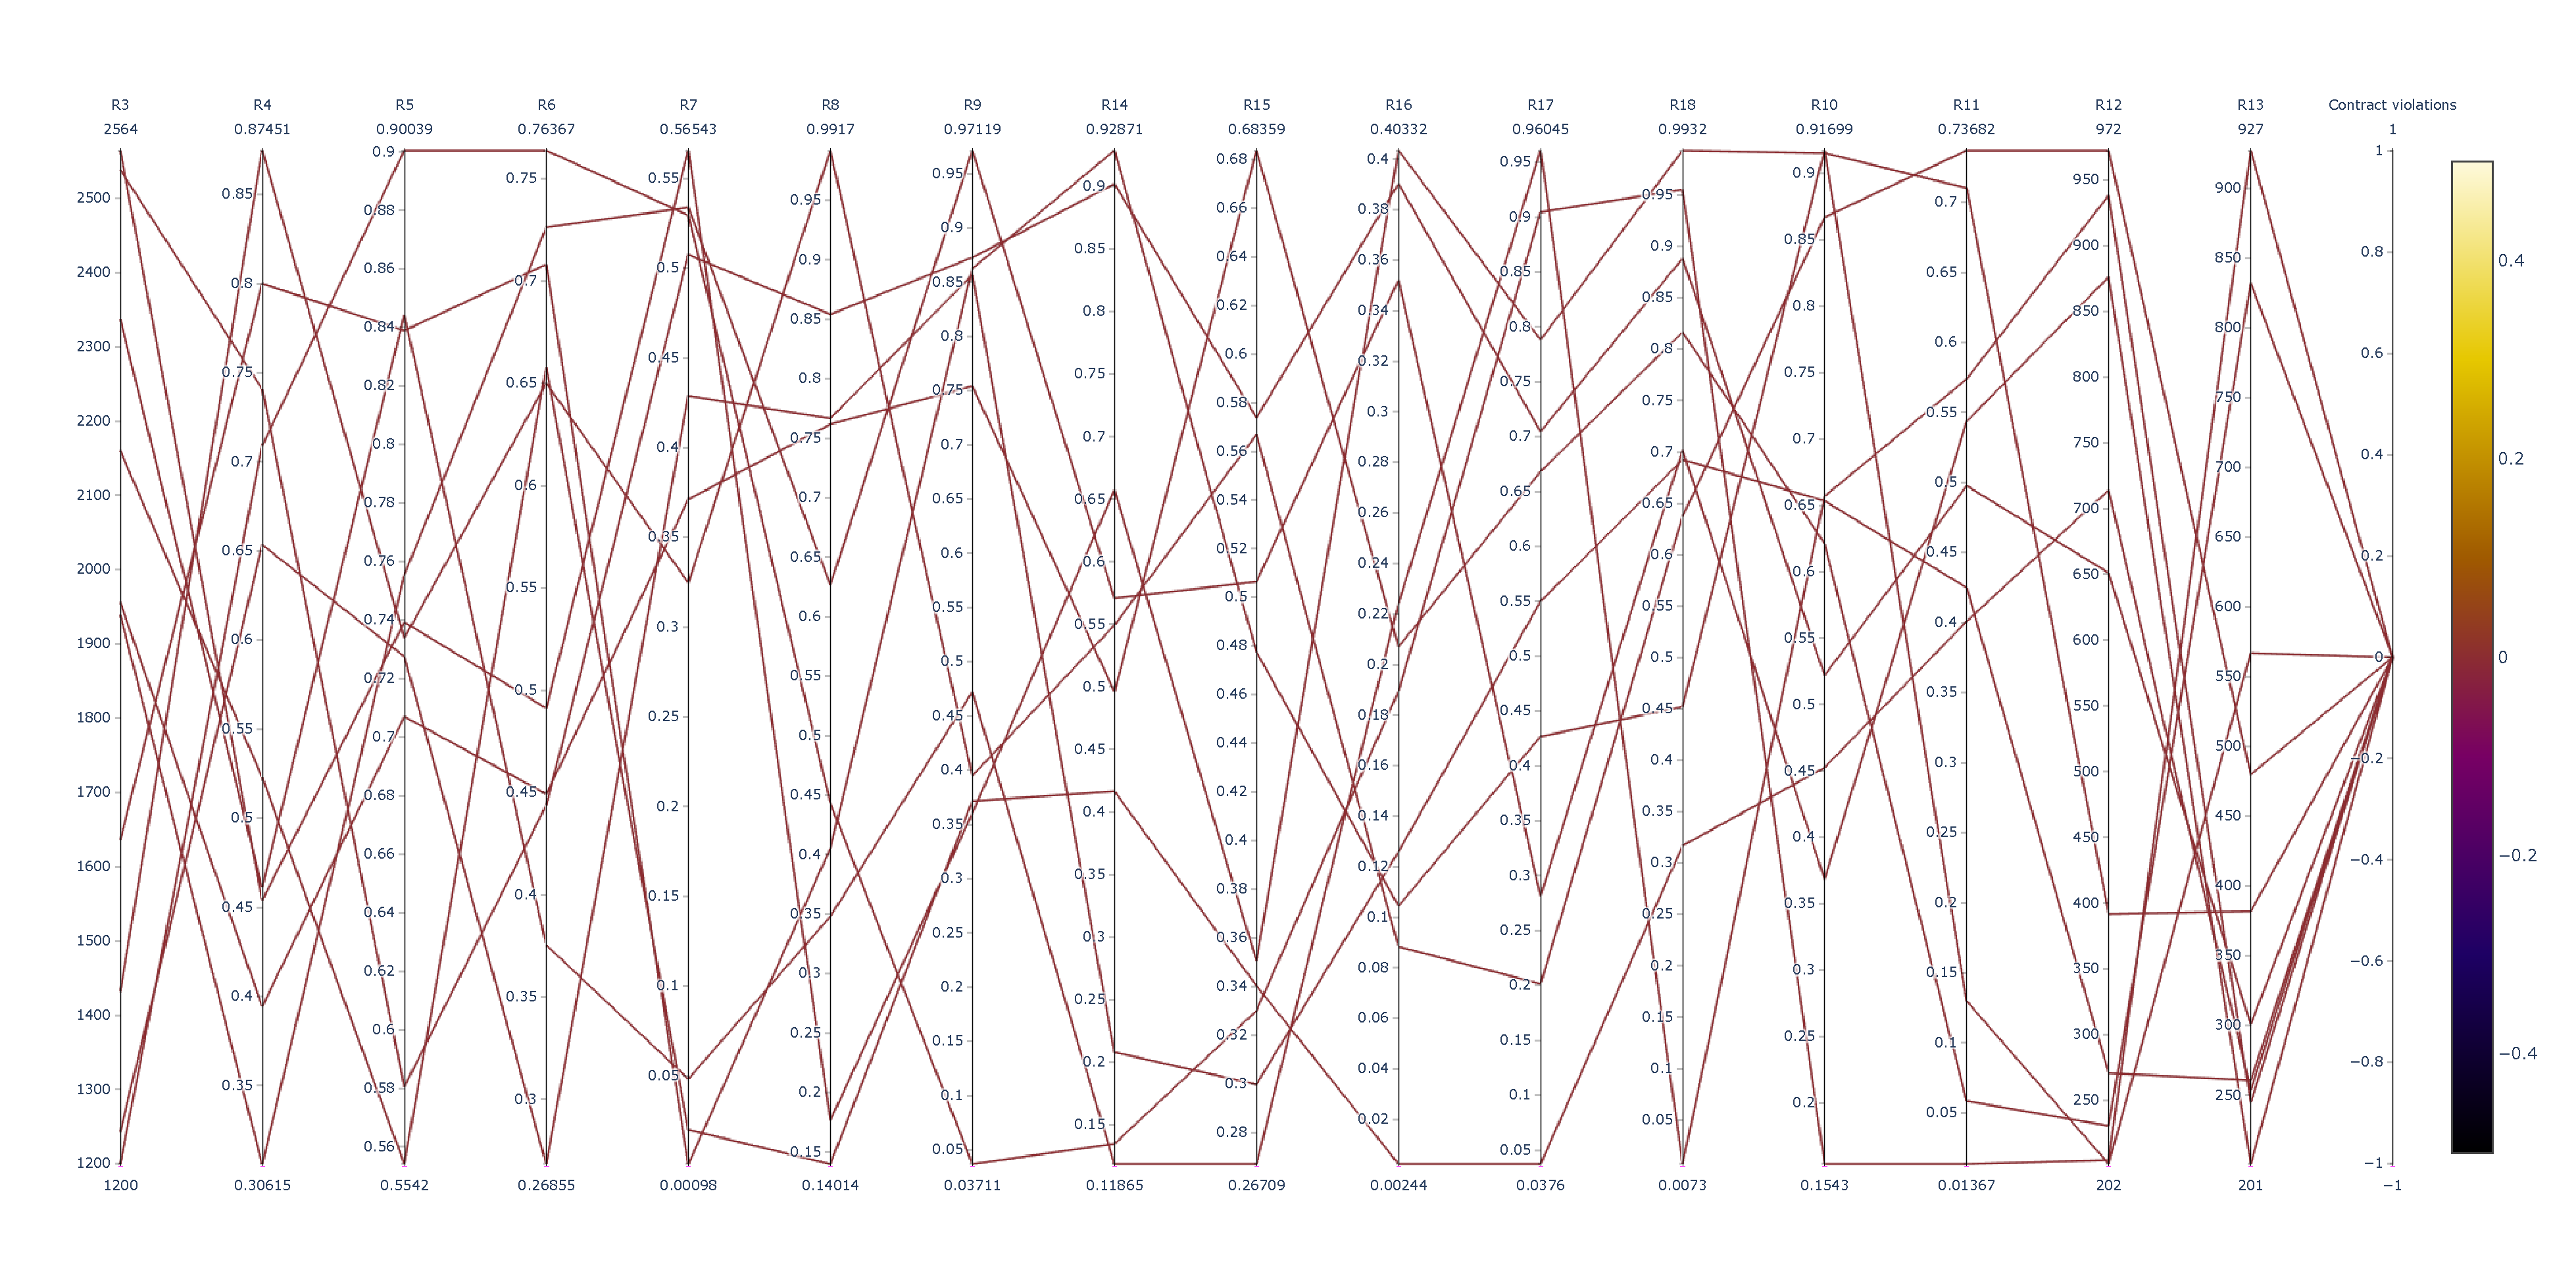
\includegraphics[width=\textwidth]{images/SPEA2_Zero_validity.html.pdf}
	\caption[]]{}
	\label{fig:SearchSpaceValid}
\end{figure}

If we are filtering out all configurations that gave not valid results, we obtained the search space with a few configurations that give valid results. A parallel plot that demonstrates this situation showed in Figure~\ref{fig:SearchSpaceValid}. The plot shows that only a few configurations give a valid result for the specified problem. However, still, there are no visible dependencies between the parameters and the number of contract violations, or between the parameters themselves.

\begin{figure}
	\centering
	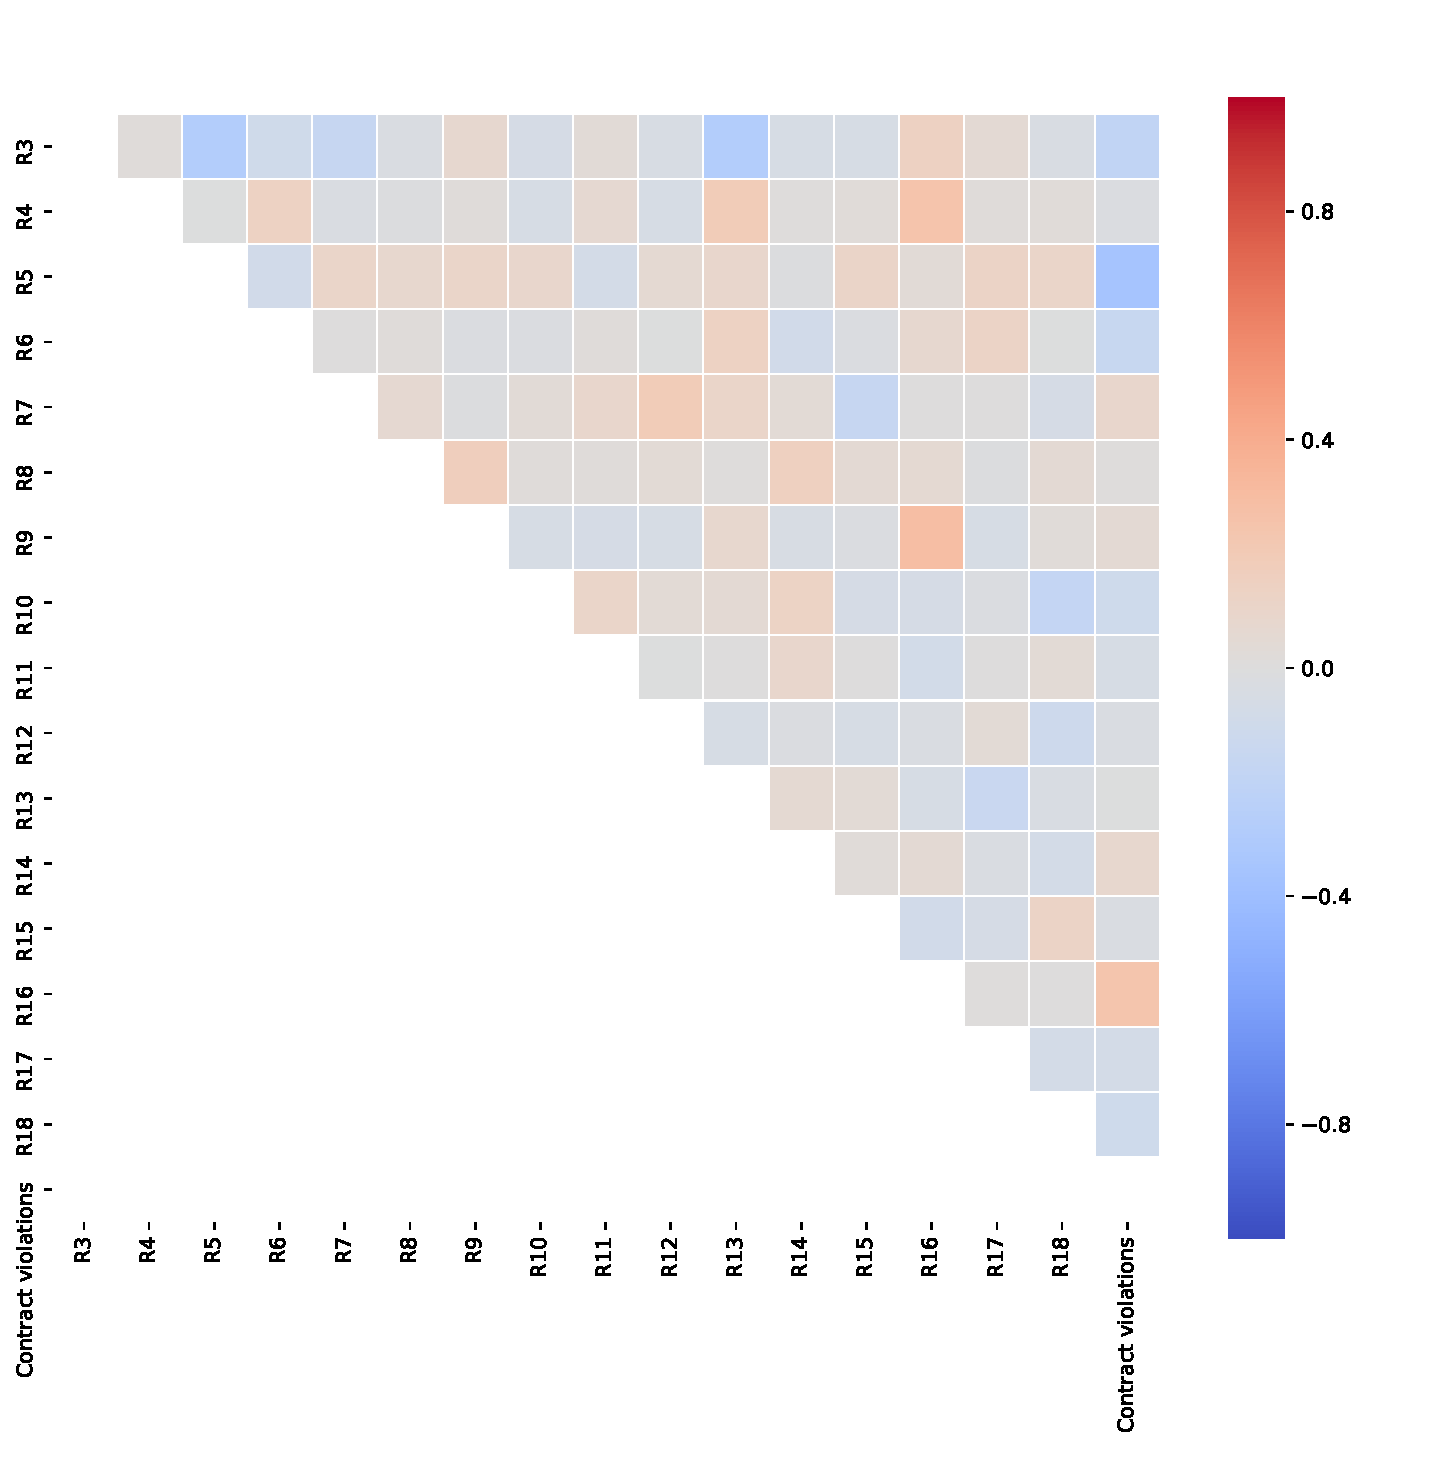
\includegraphics[width=\textwidth]{images/CorrelationAnalysis.pdf}
	\caption[]]{}
	\label{fig:CorrelationAnalysis}
\end{figure}

Cause Figure~\ref{fig:SearchSpaceViewFull} and Figure~\ref{fig:SearchSpaceValid} show that the search space view could not give any conclusions about dependencies between parameters or between parameters and number of contract violations, another method of analysis was performed.

We performed the correlation analysis of parameters to understand how are they relay on each other. The results showed in Figure~\ref{fig:CorrelationAnalysis} as a correlation matrix where the value of the correlation is the color of the cell. Each row and column in this matrix represent the parameter of the genetic algorithm. There is only an upper triangle of the matrix because it is symmetric. The last column of the matrix represents the correlation between parameters of the genetic solver (NP version) and a number of contract violations~(CVs). There are two types of correlation. Direct correlation showed with red color and an inverse correlation with blue color. In the case of the last column, direct correlation means that a bigger value o parameter gives a bigger number of contract violations. Inverse correlation, in the same case, means that the bigger value of parameter gives a smaller number of contract violations. Grey color shows that there is no correlation between values.

From the correlation analysis, we can conclude that there are no strong dependencies between the number of contract violations and parameters. There are two more important parameters: \texttt{CrossoverRate}(R5) and \texttt{CrossoverOnRandomRequestProbability}(R16).
The analysis showed that the \texttt{CrossoverRate} parameter needs to have big value and value of \texttt{CrossoverOnRandomRequestProbability} needs to be as low as possible. In this case of the small value of probability, it may be a good idea to remove this parameter for parameter tuning.

Correlation analysis showed that some parameters have dependencies. Nevertheless, we do not know yet how they depend.

For further investigation of dependencies, we constructed plots that show the distribution of parameter pairs. We will discuss only two distribution. The first plot will show one representative distribution, and the second plot represents how most of the constructed distributions look like.

\begin{figure}
	\centering
	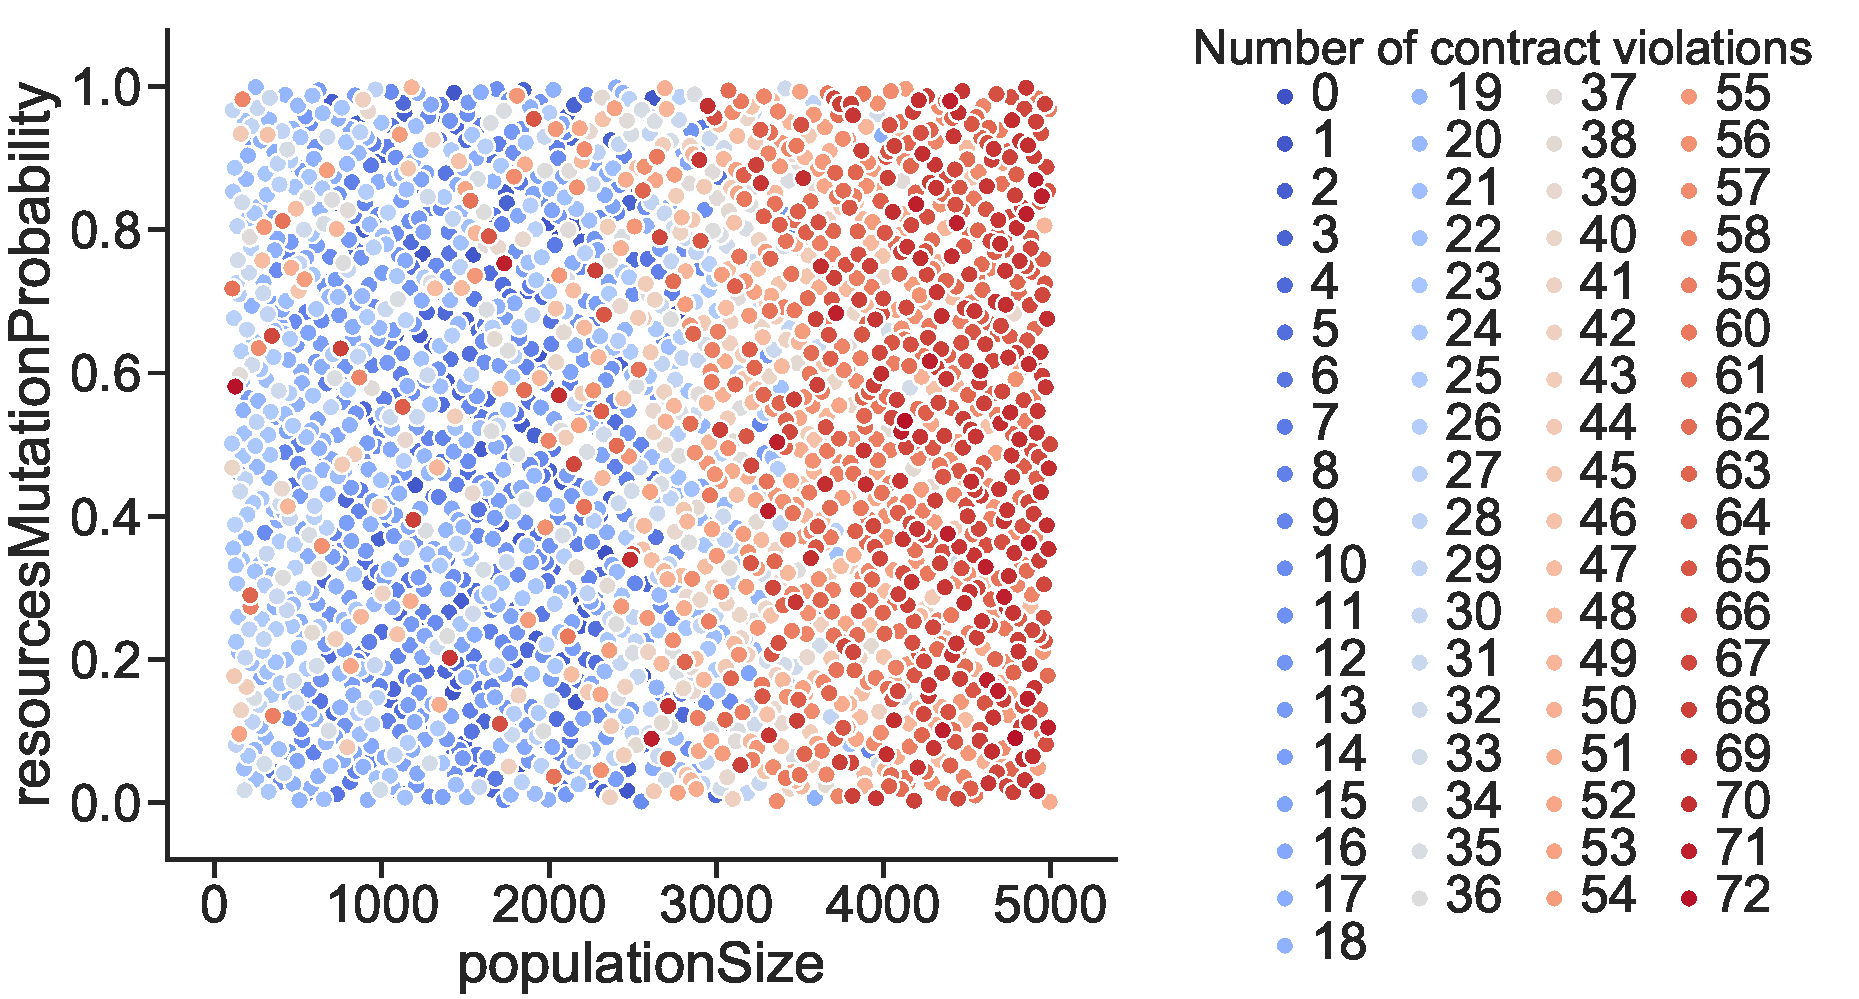
\includegraphics[width=\textwidth]{images/populatioSizeVsResMutationProbability.pdf}
	\caption[]]{}
	\label{fig:populatioSizeVsResMutationProbability}
\end{figure}

The representative distribution showed in Figure~\ref{fig:populatioSizeVsResMutationProbability}. Each point on this plot represent a value combination of two parameters \texttt{populationSize}~(R3) and \texttt{resourcesMutationProbability}~(R8). The color of the point is the number of contract violations. In this case, blue color is a small number of contract violations. Red color represents a big number of contract violations. As we can see, there is gradient coloring from the mostly blue on the left size to mostly red on the right size. Such result means that \texttt{populationSize}~(R3) have a bigger influence on the result than \texttt{resourcesMutationProbability}~(R8). The figure also shows that for any value of \texttt{resourcesMutationProbability}~(R8), there are results with any number of contract violations.

\begin{figure}
	\centering
	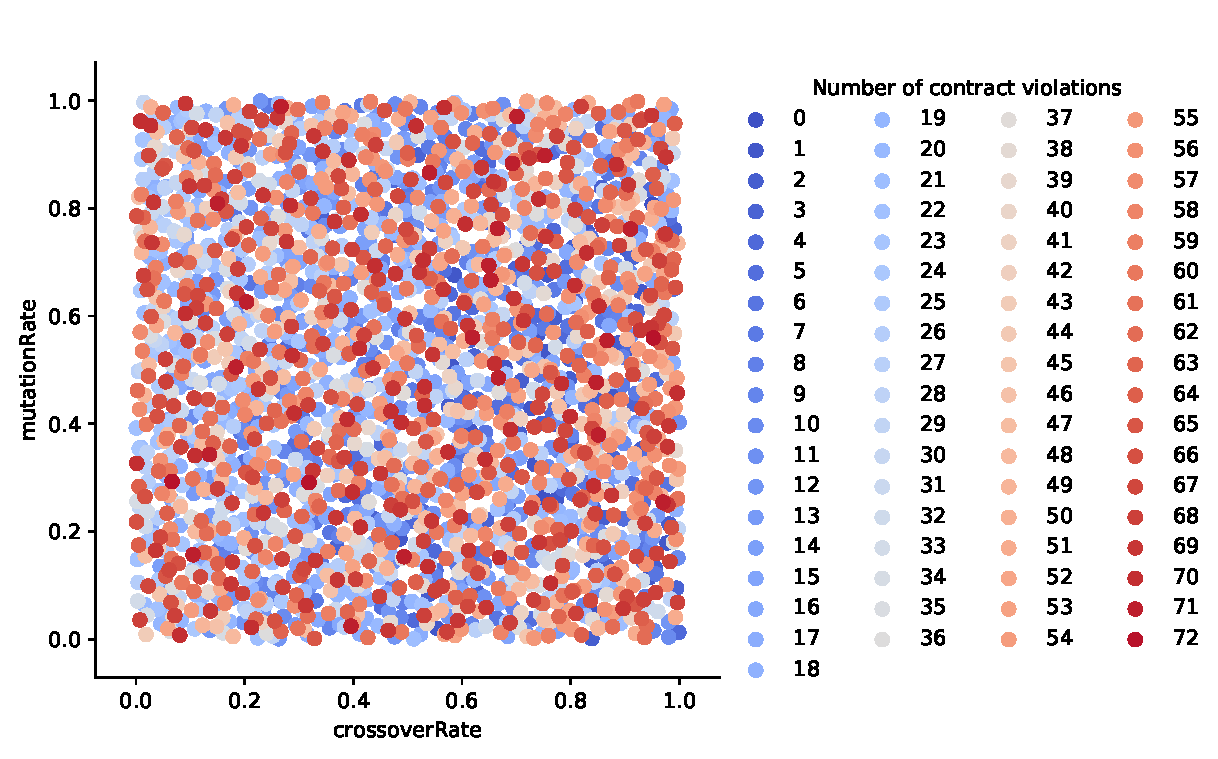
\includegraphics[width=\textwidth]{images/CrossoverRateVsutationRate.pdf}
	\caption[]]{}
	\label{fig:CrossoverRateVmutationRate}
\end{figure}

However, most distributions look like the distribution of \texttt{crossoverRate}~(R5) and \texttt{mutationRate}~(R7). It showed in Figure~\ref{fig:CrossoverRateVsutationRate}. As we can see, "good" and "bad" results exist for all values of the described parameters. That means that these parameters do not depend on each other.

Distributions of combinations of two parameters showed that some parameters have a more significant impact on the result than others. Moreover, there are parameters on the value of which the result does not depend. More examples of such distributions showed in Appendix~\ref{label}.

\begin{figure}
	\subfloat[Name A]{%
		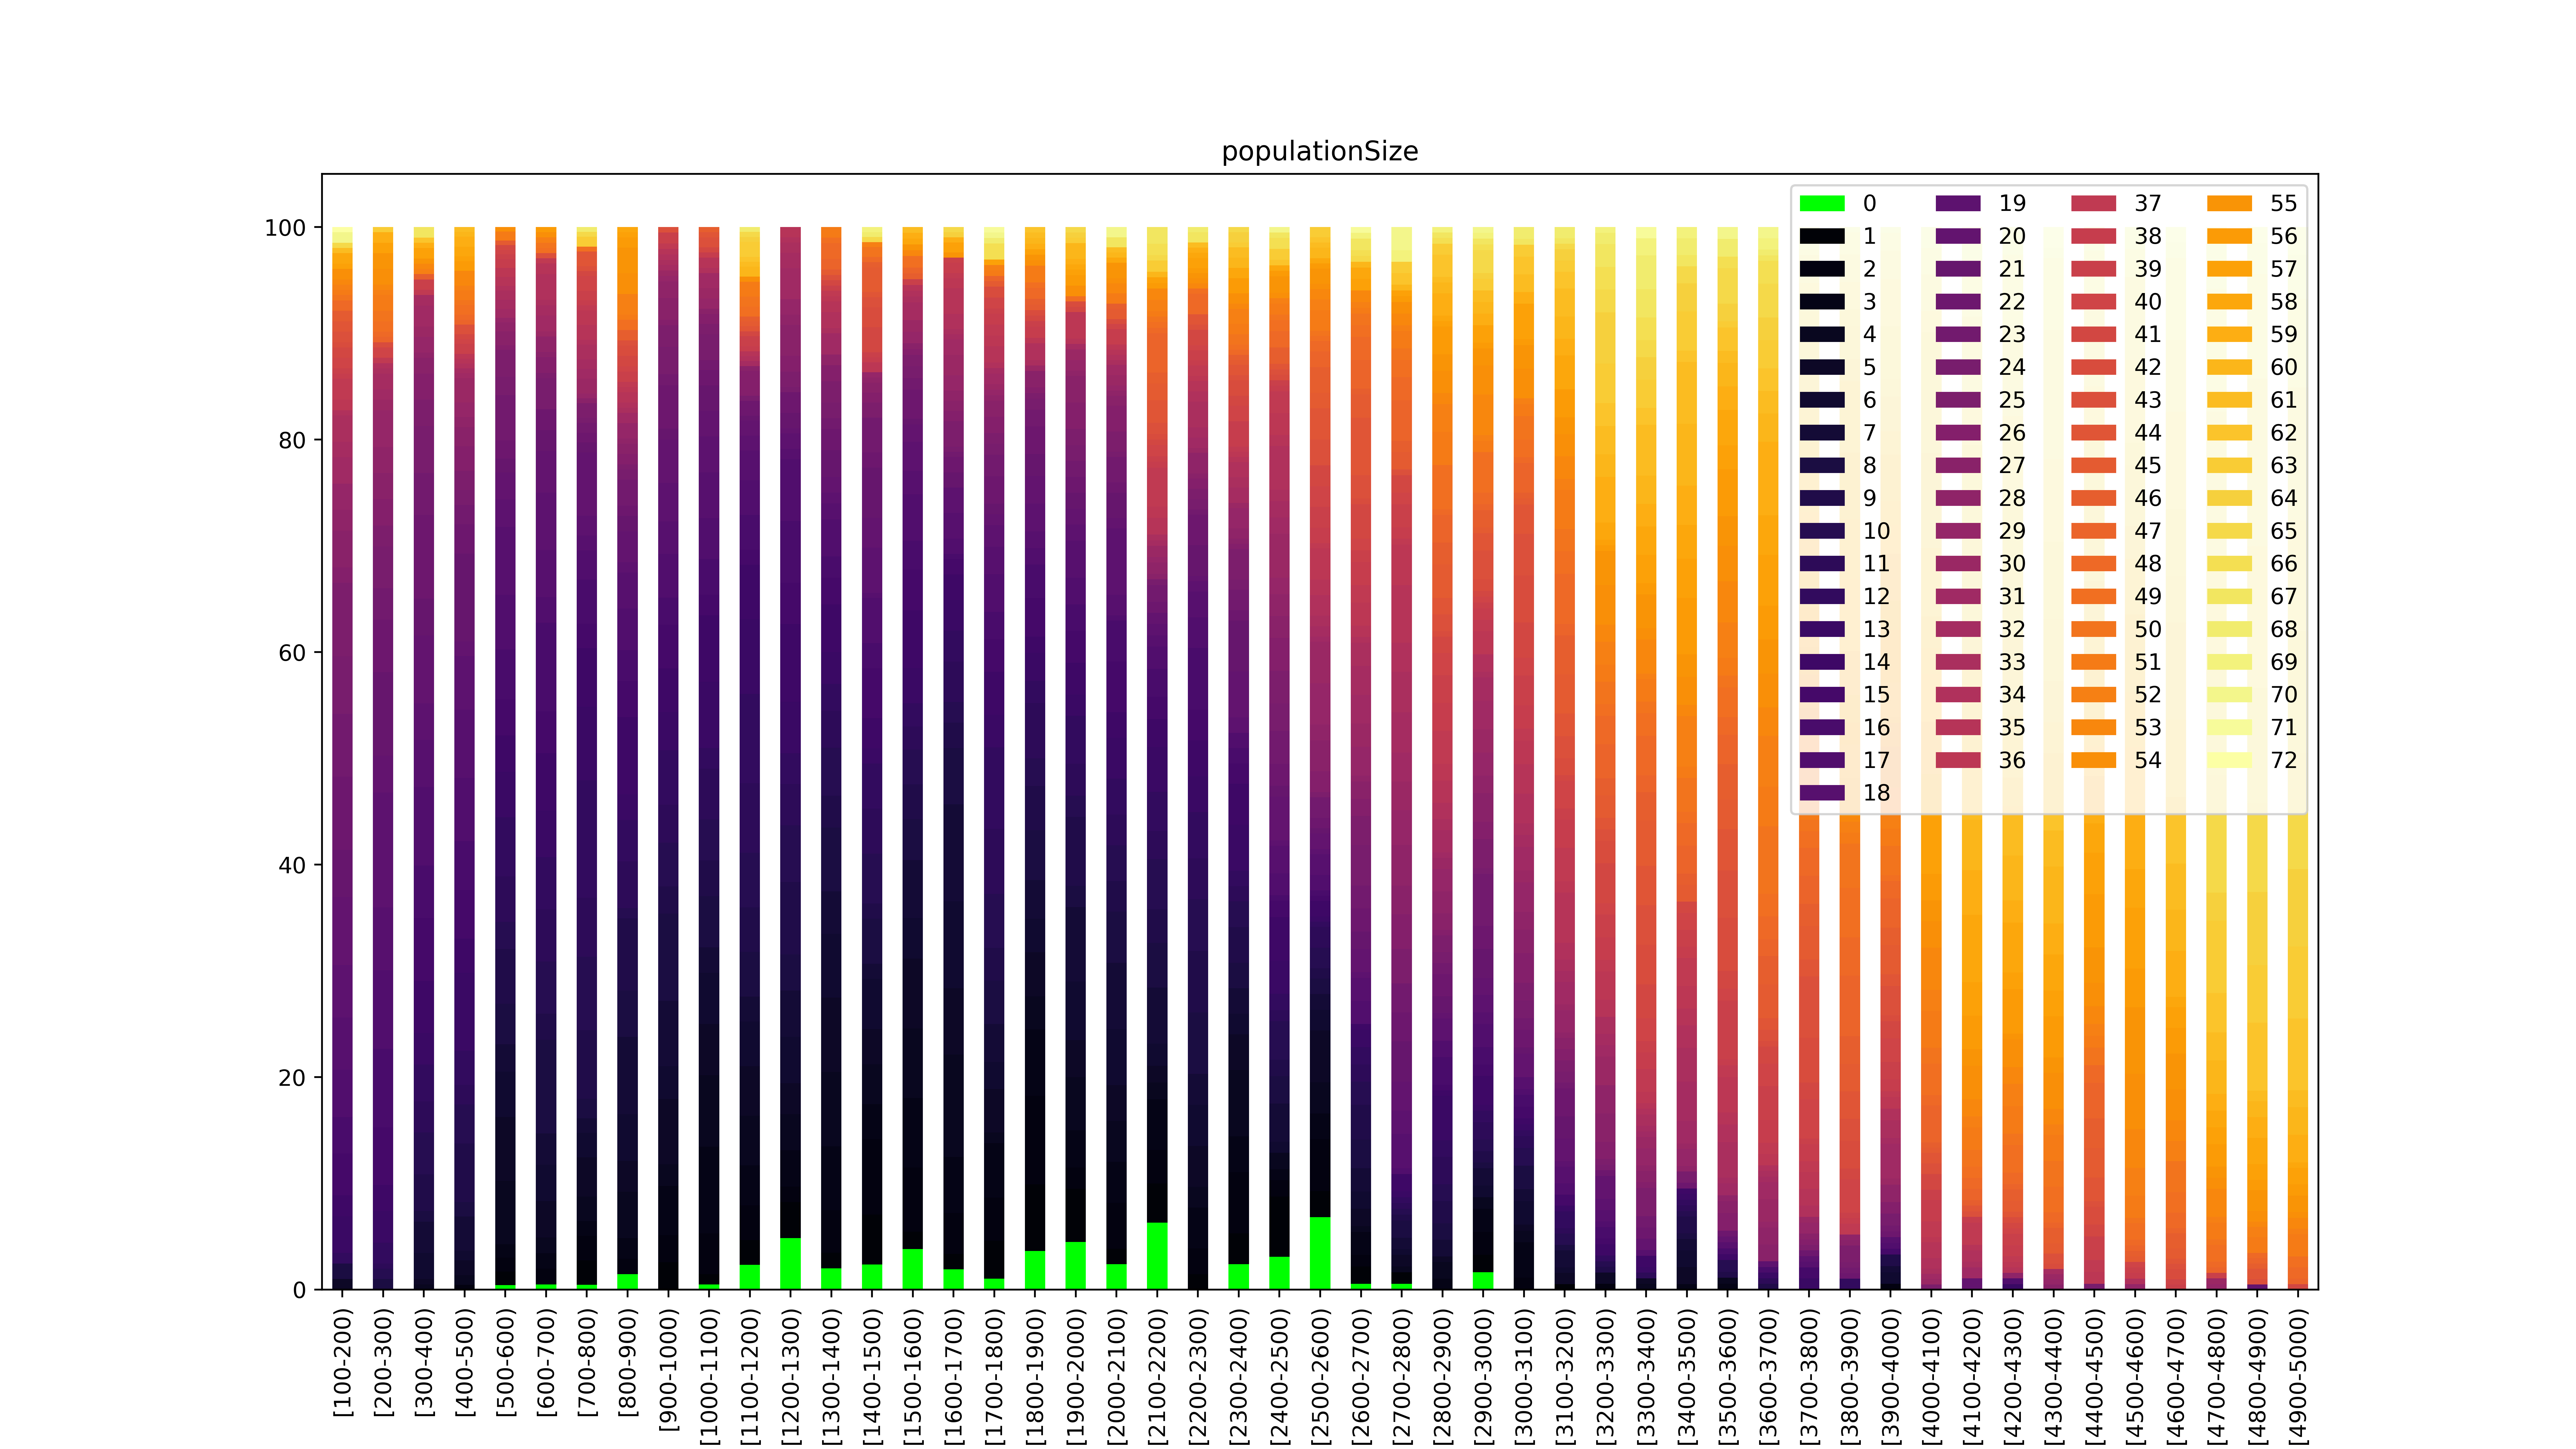
\includegraphics[clip,width=\textwidth]{images/populationSize_gradientBig.png}%
		\label{fig:populationSize_gradientBig}
	}
	
	\subfloat[Name b]{%
		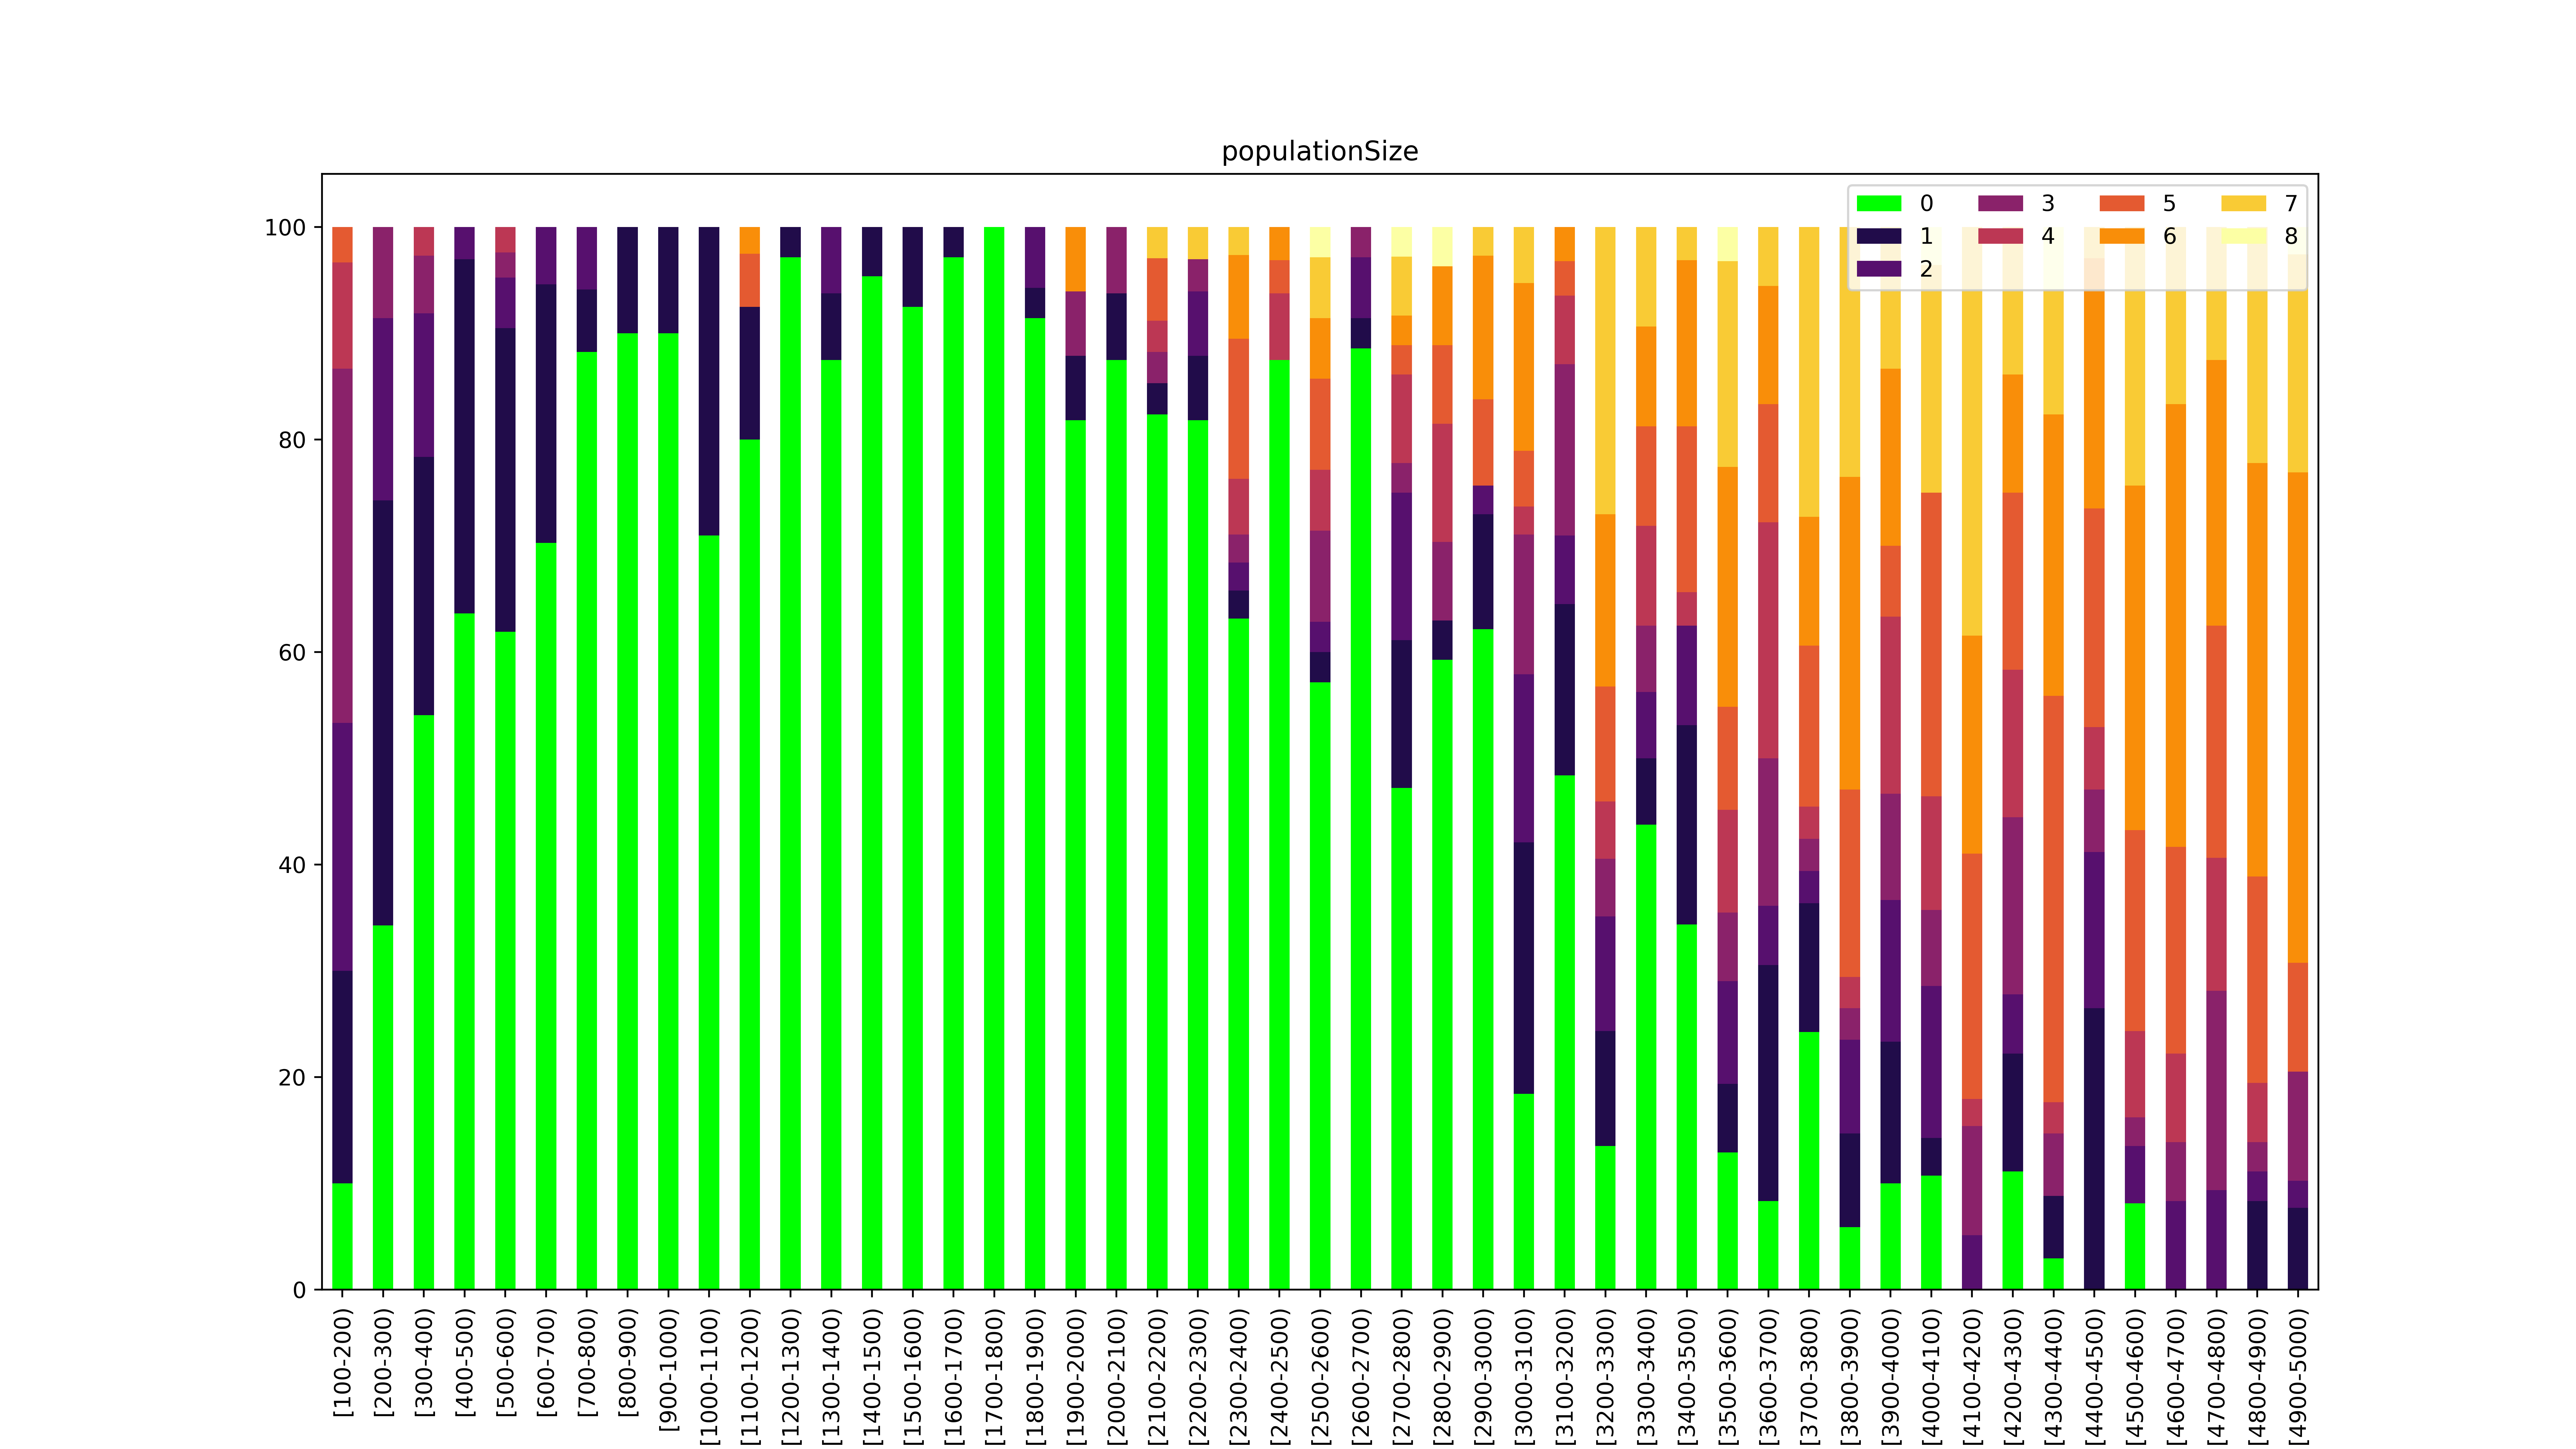
\includegraphics[clip,width=\textwidth]{images/populationSize_gradientSmall.png}%
		\label{fig:populationSize_gradientSmall}
	}
	
	\caption{main caption}
	\label{fig:populationSize_gradient}
\end{figure}

Previously discussed plots show that the results of the genetic solver depend on some parameters such as \texttt{populationSize}~(R3). So we need to analyze how the value of this parameter affects the result. Firstly we discuss the \texttt{populationSize}~(R3) parameter and the second parameter is \texttt{mutationRate}~(R7).

Figure~\ref{fig:populationSize_gradientBig} shows the distribution of the \texttt{populationSize}~(R3) parameter values and the number of contract violations that this value could give. The X-axis is a set of ranges of values for the parameter \texttt{populationSize}~(R3). Each range consists of 100 values. All ranges are sorted. A normalized bar is built for each range. Each bar consists of segments of different heights and colors. The segment color shows the number of contract violations, where black is one violation, and yellow is a large number of violations. The green color of the segment indicates valid results(zero contract violations). The segment height of one color means a percentage of the total number of configurations that have the same parameter value and which give the result with the same number of contact failures.

This distribution shows that the left side and the central part of the plot give a smaller number of contract violations because sectors have mainly dark colors and green color. The right side of the distribution contains higher values of the parameter. Moreover, solutions with those values give more contract violations. As can be seen, valid solutions located in the range from 1000 to 2600.

For a more visual image, we construct a similar graph for the smaller problem. This problem described with parameters:
\begin{itemize}
	\item Software variants: 2,
	\item Number of requests: 2,
	\item Component tree depth: 2,
	\item Resources ratio: 5,
	\item timeout to solve the problem: 5 minutes.
\end{itemize}

It is shown in Figure~\ref{fig:populationSize_gradientSmall}. If we compare Figure~\ref{fig:populationSize_gradientSmall} and Figure~\ref{fig:populationSize_gradientBig}, we can see that they have a similar distribution.

The second  discussed parameter is \texttt{mutationRate}~(R7). The distribution of values of this parameter showed in Figure~\ref{fig:mutationRate_gradient}. For better visual understanding, the distribution is built for a smaller problem described above. 
As we can see, the percentage of valid results for any described range of values of the \texttt{mutationRate}~(R7) parameter varies from 50 to 60. The distributions of most parameters look like the distribution described here. Such a distribution means that the result of the genetic solver does not depend on the value of the parameter. 

\begin{figure}
	\centering
	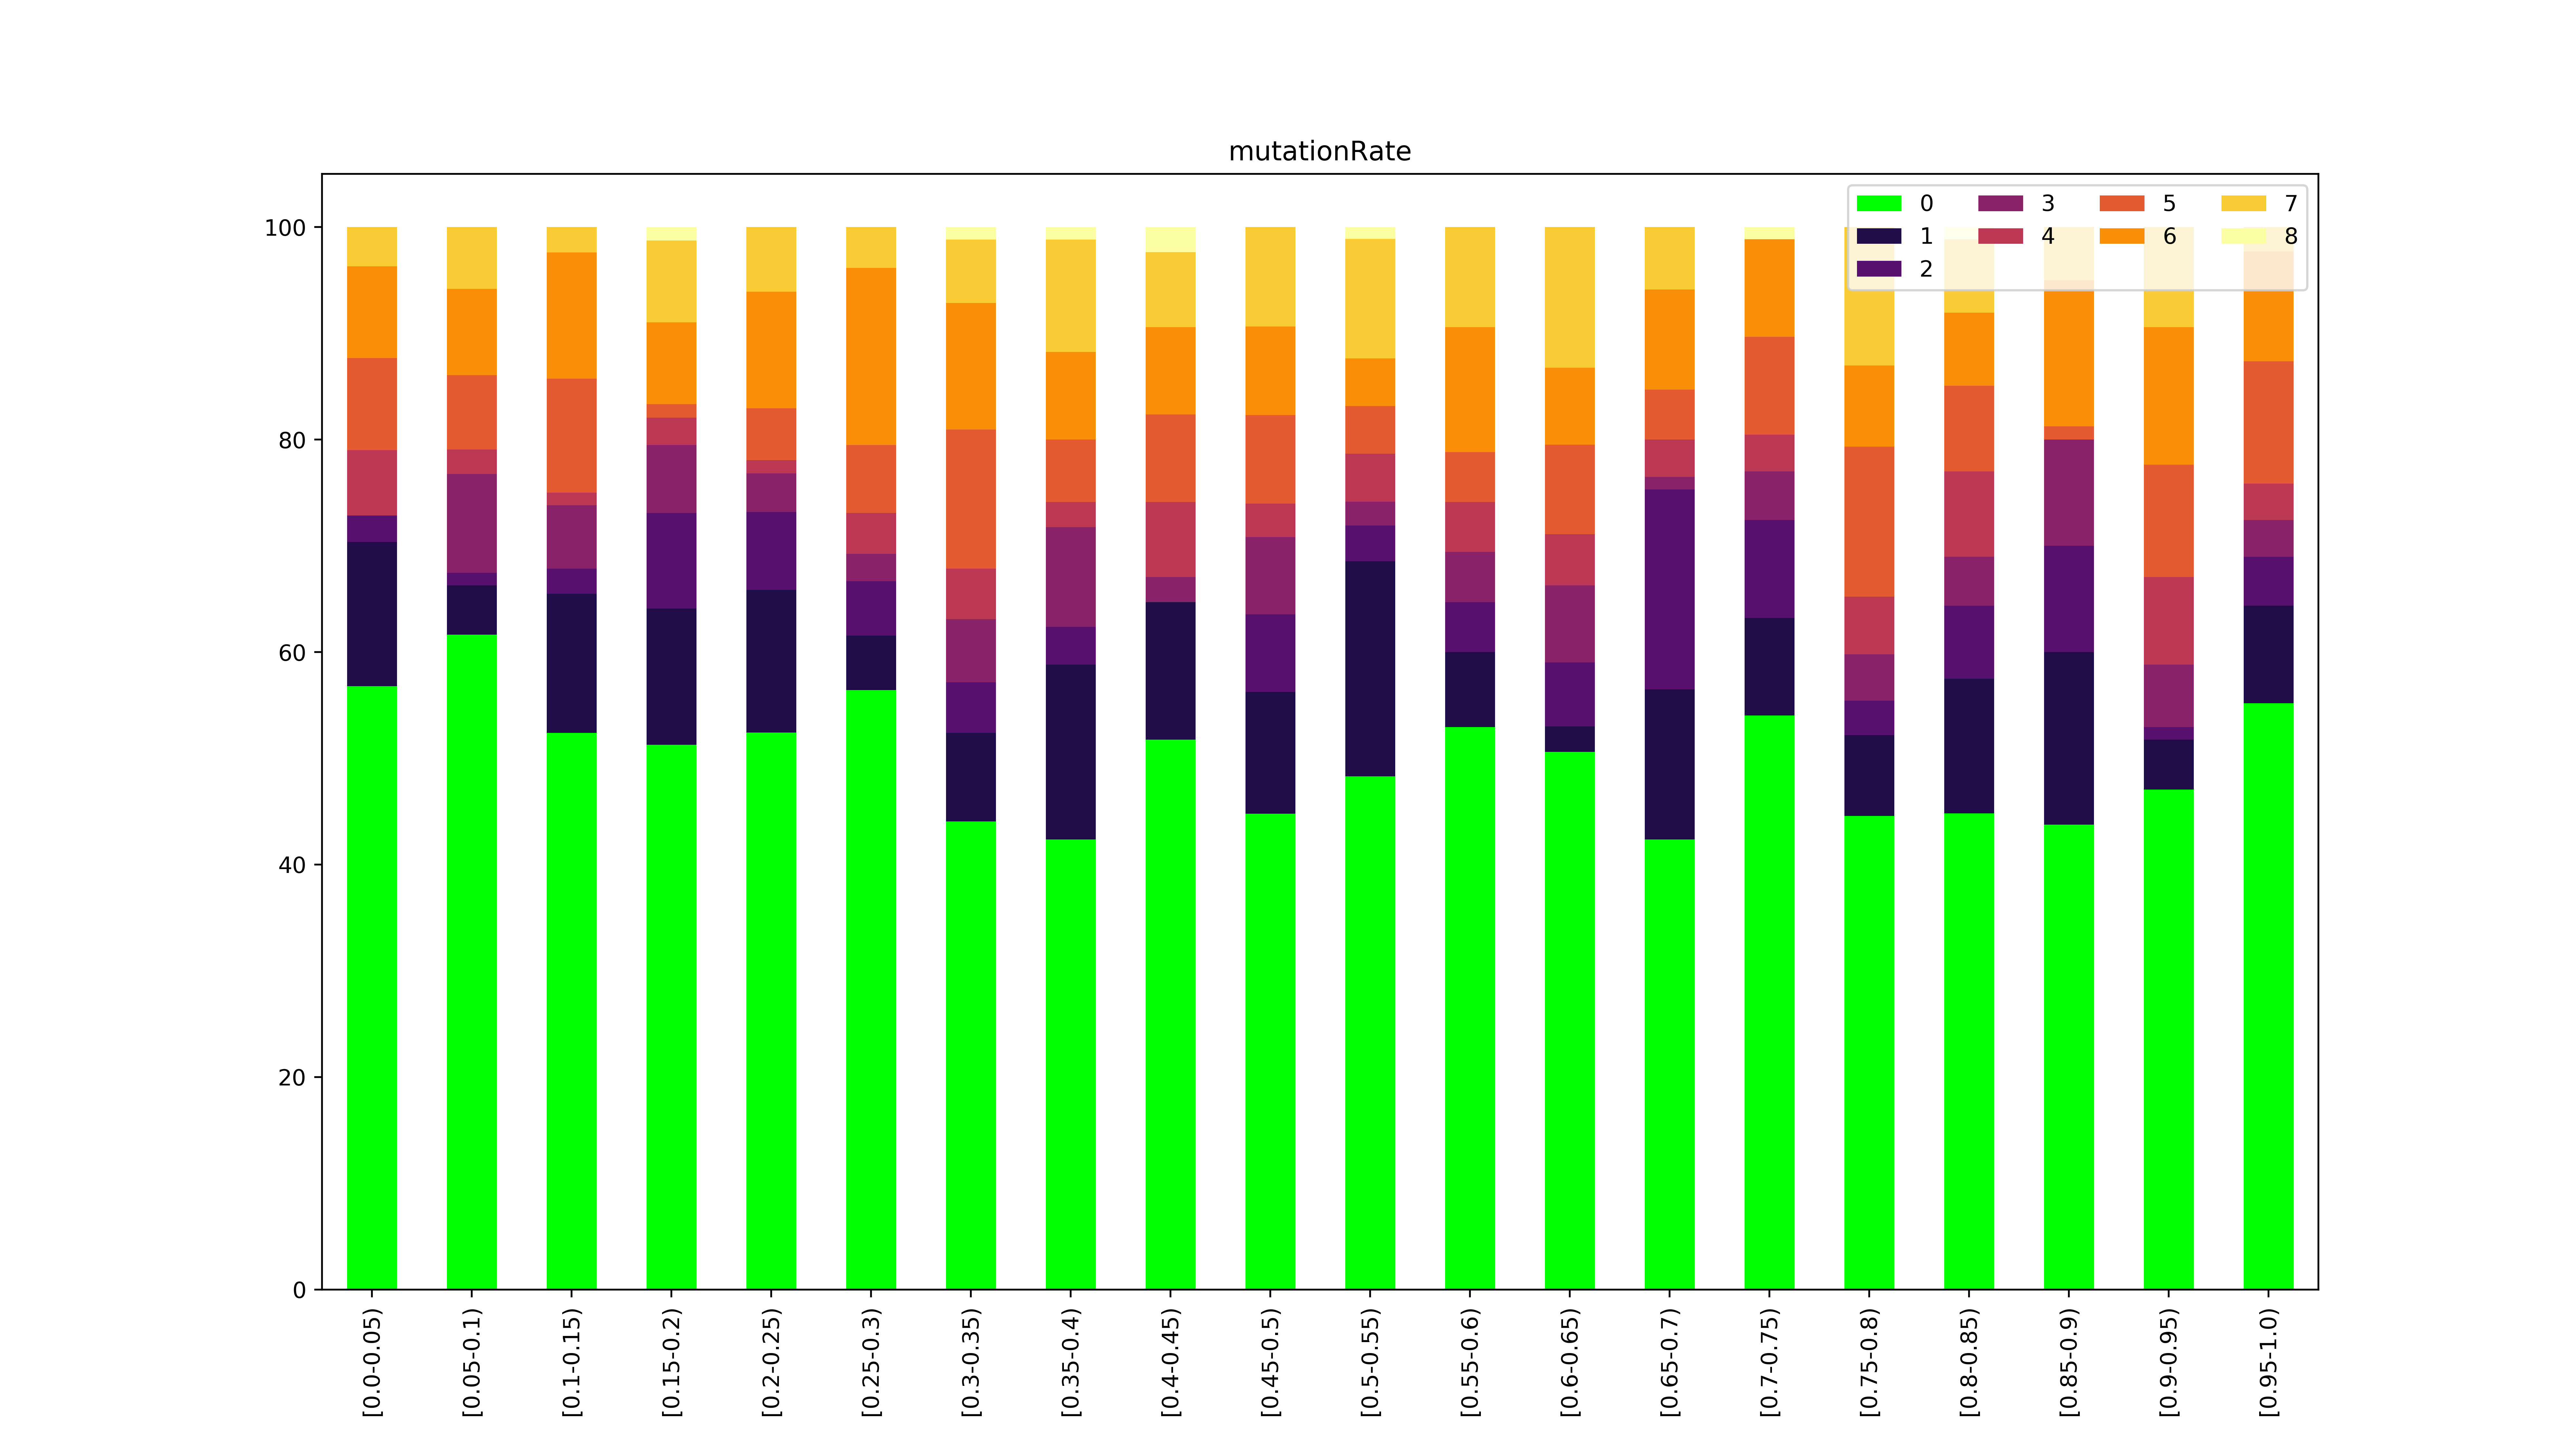
\includegraphics[width=\textwidth]{images/mutationRate_gradient_500dpi.png}
	\caption[]]{}
	\label{fig:mutationRate_gradient}
\end{figure}

The two types of distribution of parameter value and number of contract violation were discussed. Distributions for both problems for each parameter presented in Appendix\ref{label}. These plots confirm the conclusions that we made above. Values of some parameters such as \texttt{populationSize}~(R3), \texttt{crossoverRate}~(R5), \texttt{populateSoftwareSolutionAttempts}~(R13) and \texttt{crossoverOnRandomRequestProbability}~(R16) have a higher effect on the result.
The distribution  of the \texttt{crossoverOnRandomRequestProbability}~(R16) parameter showed in Appendix~\ref{label} confirms conclusions from correlation analysis that lower value gives better result. 
Some parameters give "good" and "bad" results for all values. That means that we could remove them from the parameter tuning and use constant value. Furthermore, for other parameters, values ranges could be adjusted.

To answer the question of what value of parameters with no obvious advantage in distribution, we construct a similar distribution with the quality of the solution.
As earlier we presented two distribution for \texttt{populationSize}~(R3) and \texttt{mutationRate}~(R7) parameters for smaller problem for smaller problem.

Figure~\ref{fig:populationSizeObjective} shows the quality distribution for the \texttt{populationSize}~(R3). This distribution differs from the previous one shown in Figure~\ref{fig:populationSize_gradientSmall} that all non-valid configurations are located in one segment that marked as "non-valid" and have a black color. Valid results consist of segments with different high and color. Each segment represents the percentage of the total number of configurations that have the same parameter value and which give the result near the same quality. All colors except black show the deviation of the quality of the solution from optimum in percent. Greed color represents optimal solutions.

As we can see, if a genetic solver gets valid results, the quality of the solution is optimal, or near-optimal. This distribution also confirms conclusions in Section~\ref{sec:evaluation}.

For current analysis the distribution of the \texttt{mutationRate}~(R7) parameter is more interesting and it showed in Figure~\ref{fig:mutationRateObjective}. The distribution of contract violations shows that any value of the parameter could give a valid result. However, the distribution of quality shows that some values of the parameter could give an optimal solution to the problem. Let us compare two ranges of values [0.45, 0.5) and [0.75, 0.8). Both ranges have near the same percentage of valid results of 50\%.
Nevertheless, the first range could give an optimal solution. The second range could not give such a solution. Moreover, the percentage of near-optimal solutions for the second range is lower.


\begin{figure}
	\centering
	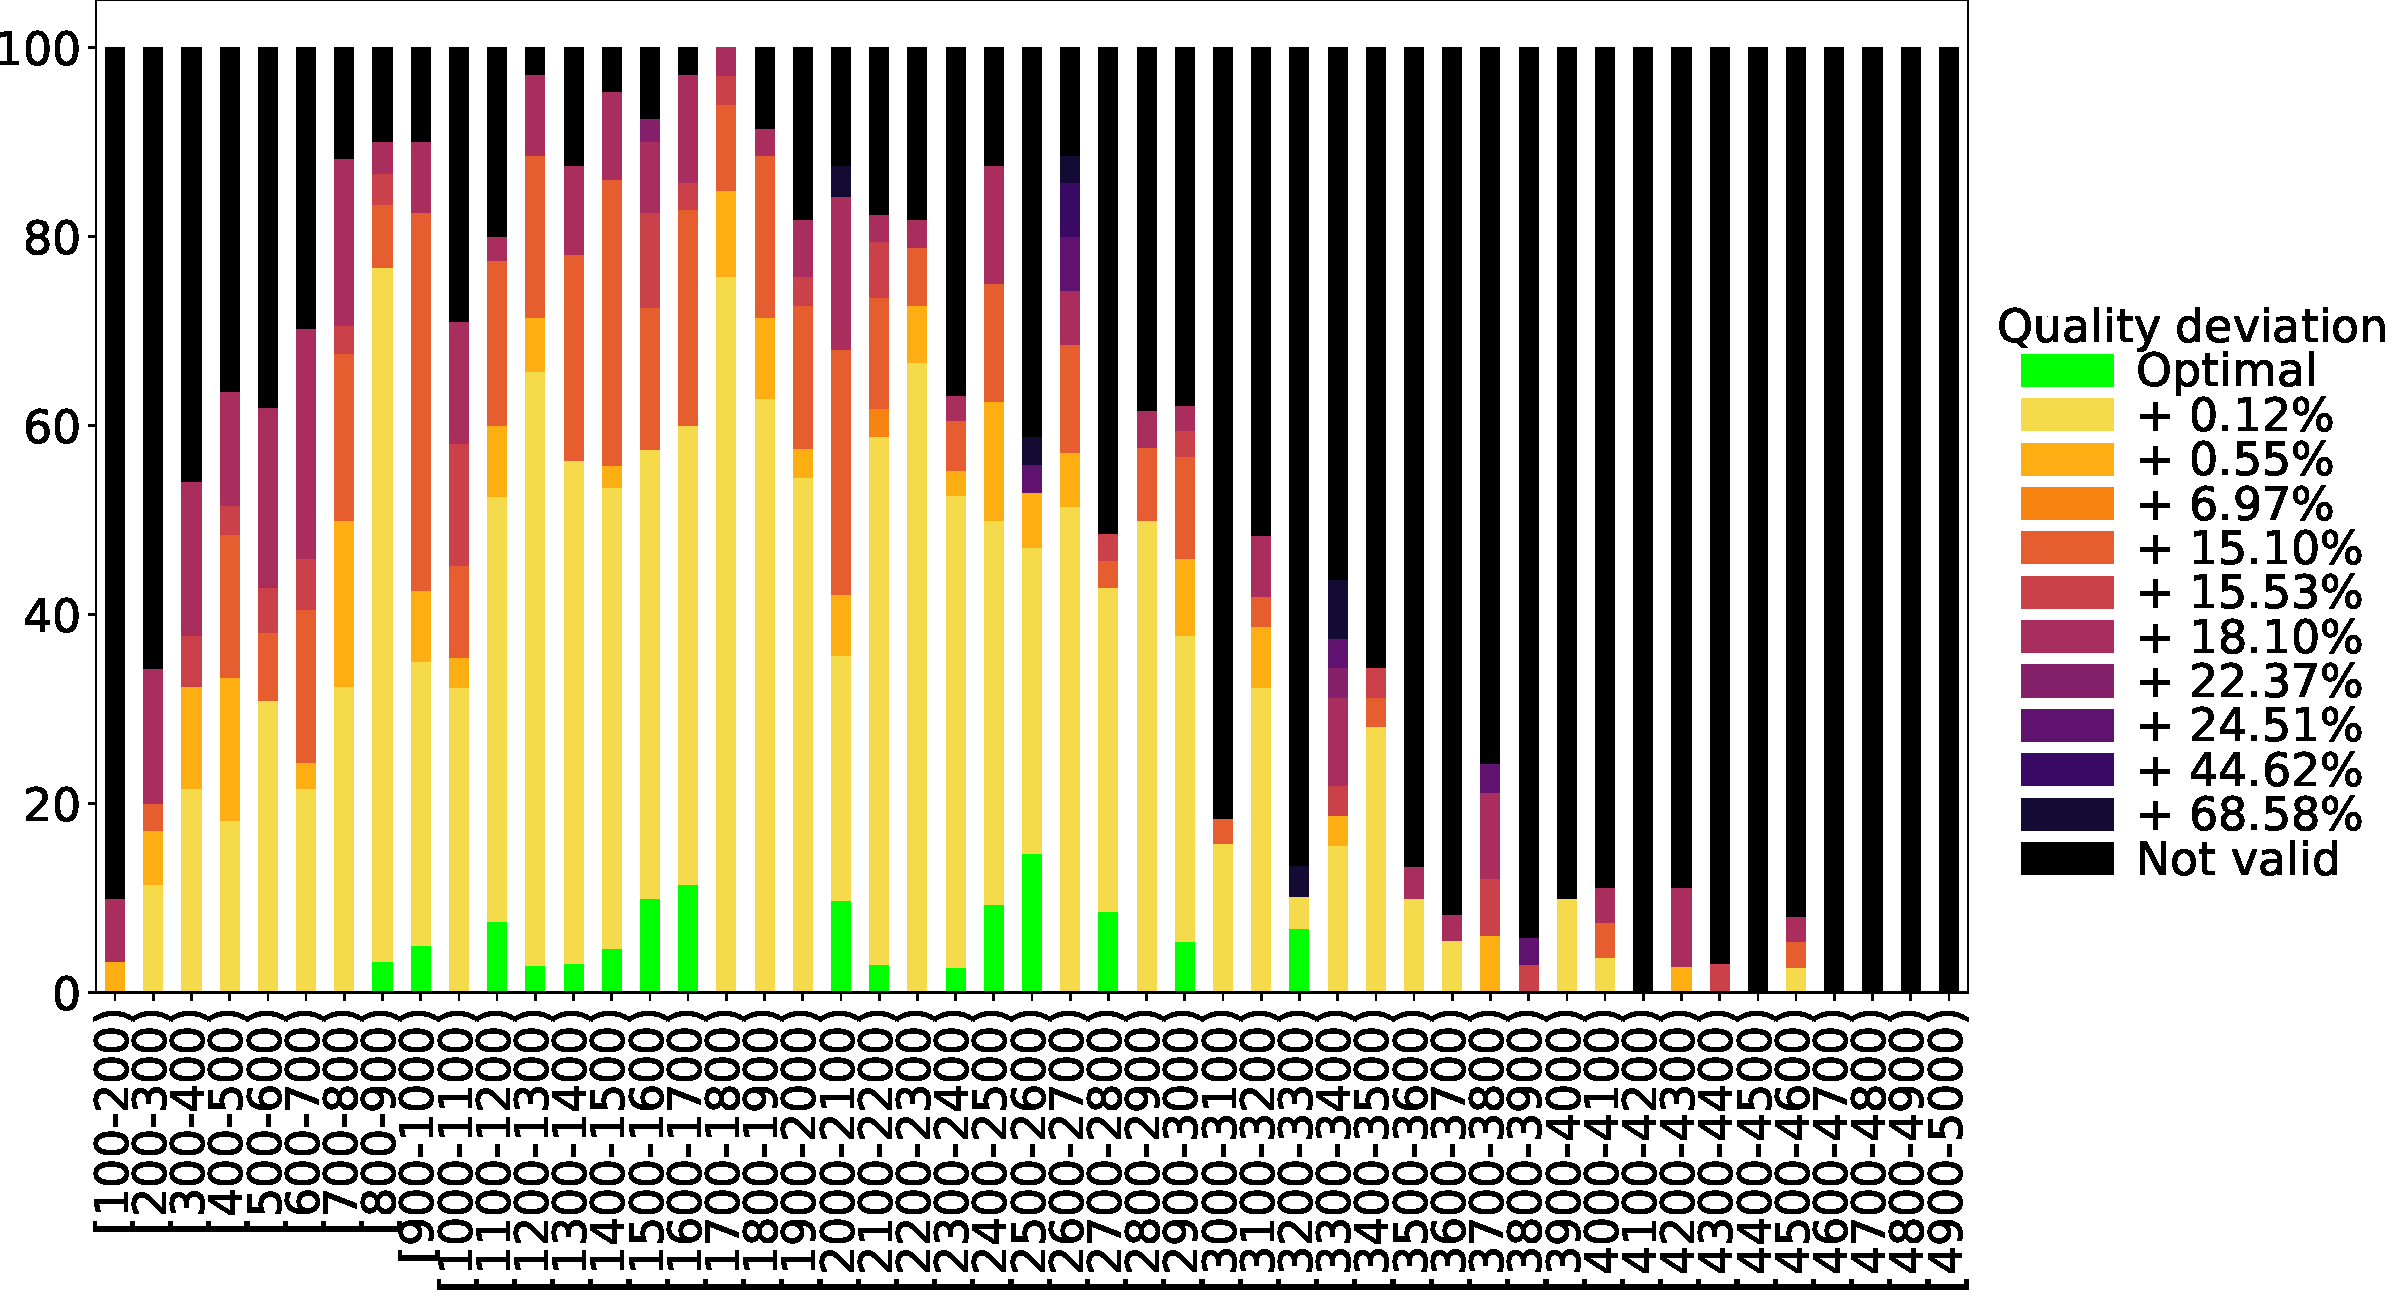
\includegraphics[width=\textwidth]{images/populationSizeObjective.pdf}
	\caption[]]{}
	\label{fig:populationSizeObjective}
\end{figure}


\begin{figure}
	\centering
	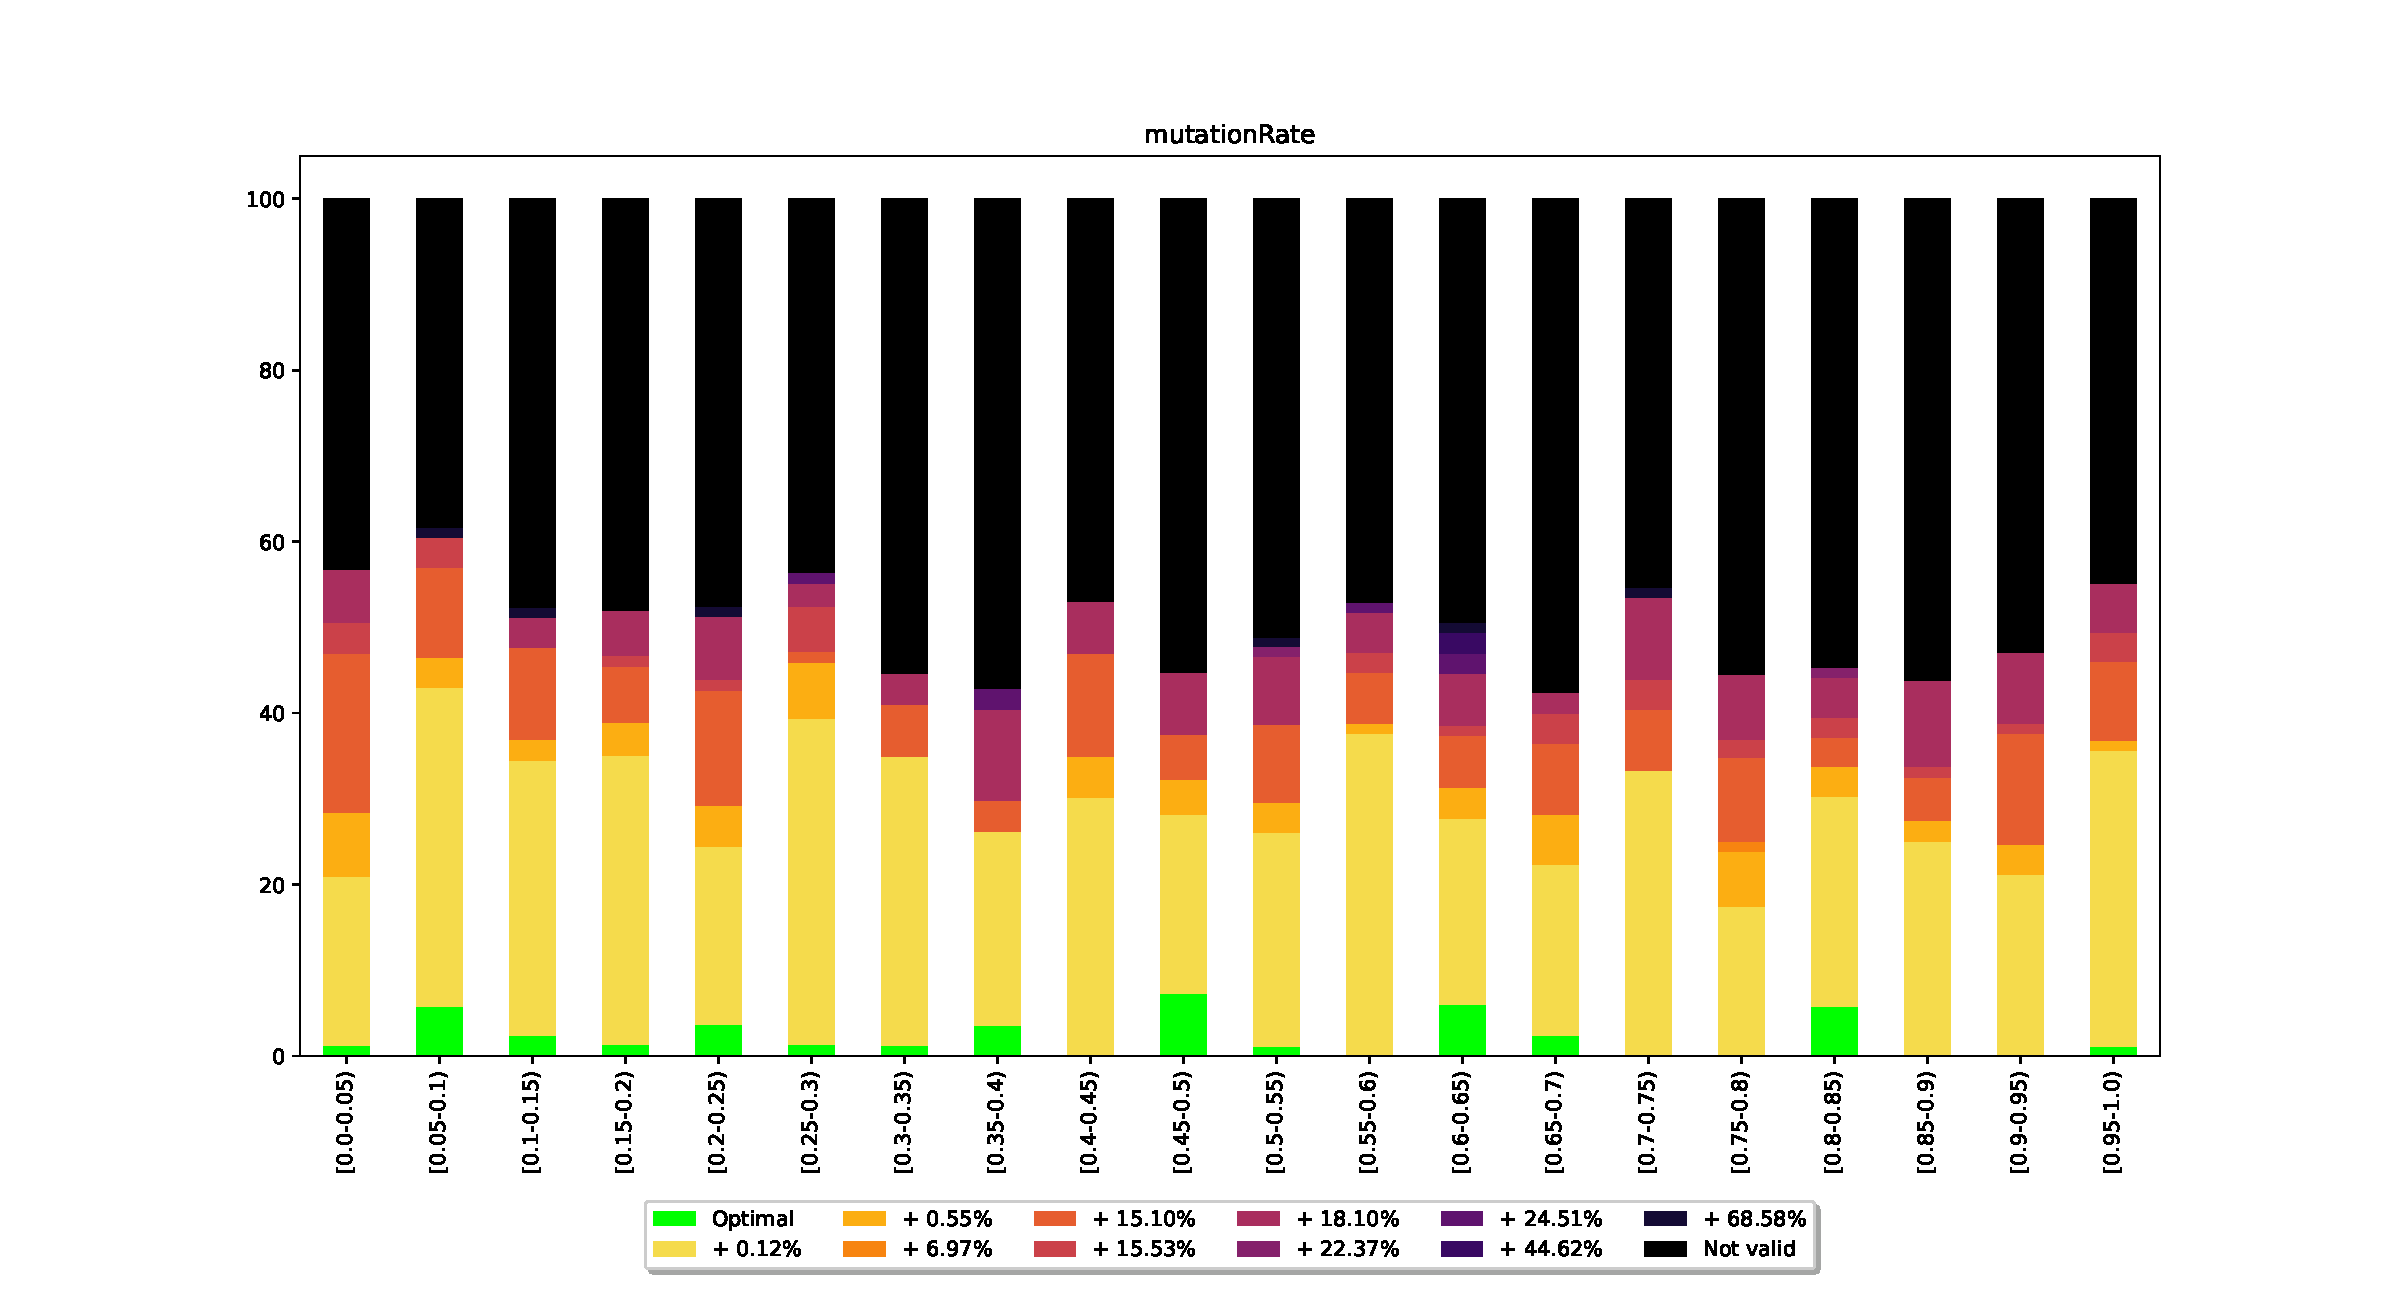
\includegraphics[width=\textwidth]{images/mutationRateObjective.pdf}
	\caption[]]{}
	\label{fig:mutationRateObjective}
\end{figure}

Last discussed plots shows that validity of the result that described as a number of contract violation could not depend on the value of the parameter. However, the quality of the solution depends on the parameter value. As a conclusion, we could say that we could remove some parameters from the parameter tuning if our goal is to find a valid solution. But if we are looking for the best quality of the solution, it needs all the parameters. This fact shows that multi-objective optimization is a complex question.